

% Dies ist die Preambel
% \documentclass[12pt,a4paper,bibtotoc, twoside, cleardoublepage=empty]{article} % twoside
\documentclass[12pt,a4paper,bibtotoc, cleardoublepage=empty]{article}  

% How to make citations appear within square brackets [ ] instead of parentheses ( )?
% https://tex.stackexchange.com/questions/82570/how-to-make-citations-appear-within-square-brackets-instead-of-parentheses



\usepackage{pdfpages} % import pdf
% Highlighting
\usepackage[cache=false]{minted}

% Make Listings, Figures and Tables share the same counter
\makeatletter
\AtBeginDocument{%
  \let\c@figure\c@listing
  \let\thefigure\thelstlisting
  \let\c@table\c@listing
  \let\thetable\thelstlisting
  \let\ftype@lstlisting\ftype@figure % give the floats the same precedence
  \let\ftype@table\ftype@figure % give the floats the same precedence
}
\makeatother
% End - Make Listings, Figures and Tables share the same counter

% das ist Standard - nie ohne aus dem Haus gehen
%\usepackage[german]{babel}
% Biber!!!!!!!!!!!!!!!!!!

% How do I ensure that figures appear in the section they're associated with? https://tex.stackexchange.com/questions/279/how-do-i-ensure-that-figures-appear-in-the-section-theyre-associated-with
\usepackage[section]{placeins}

\usepackage{ebgaramond}

\usepackage{typearea}
\usepackage[style=authortitle]{biblatex}

%englisch
\usepackage[american]{babel}
\usepackage[utf8]{inputenc}
%german
%\usepackage[babel,german=guillemets]{csquotes}
% oneside centered
%\bibliographystyle{plain}

\setcounter{biburllcpenalty}{7000}
\setcounter{biburlucpenalty}{8000}
\bibliography{lit/literatur}



\usepackage[onehalfspacing]{setspace}

\usepackage{tabularx} % in the preamble

% Fu�noten auch in �berschriften
\usepackage[stable]{footmisc}

% Bilder
\usepackage{graphicx}
\graphicspath{ {../img/} } 
\usepackage{float} 

% Seitenraender 
\usepackage{geometry}

%\geometry{a4paper, top=20mm, left=35mm, right=20mm, bottom=20mm,headsep=12mm, footskip=12mm} % twoside
\geometry{a4paper, top=20mm, left=20mm, right=20mm, bottom=20mm,headsep=12mm, footskip=12mm} % oneside centered


%\usepackage{natbib}


%Hinweisbox
\usepackage{calc}
\usepackage{hhline} 
\usepackage{multirow} 
\usepackage{xcolor}
\usepackage{colortbl}
\usepackage{graphicx}

\newlength{\iconwidth}
\setlength{\iconwidth}{1cm}

\definecolor{boxheadcol}{gray}{.6}
\definecolor{boxcol}{gray}{.9}

\newenvironment{displaybox}[2]{%
  \begin{center}
    \setlength\arrayrulewidth{0.75pt}%
    \arrayrulecolor{white}%
    \renewcommand{\arraystretch}{1.3}%
    \begin{tabular}{p{\iconwidth}p{\linewidth-4\tabcolsep-\iconwidth}}
      \multirow{2}{*}{#2}&\cellcolor{boxheadcol}\textbf{\sffamily\color{white}#1} \\%
      \hhline{~-}%
      &\cellcolor{boxcol}%
}{%
      \\
    \end{tabular}
  \end{center}%
}


\newenvironment{Tipp}{%
\begin{displaybox}{Tipp}{
\includegraphics[width=\iconwidth]{img/com/icon-tipp}}}%
{\end{displaybox}}

\newenvironment{Hinweis}{%
\begin{displaybox}{Hinweis}{
\includegraphics[width=\iconwidth]{img/com/icon-hinweis}}}%
{\end{displaybox}}
%Hinweisbox ende

% Standart Kopfzeile 
\pagestyle{headings}
  
% Referenzen

\usepackage{hyperref}
\hypersetup{
  colorlinks=true,
  linkcolor=black,
	citecolor=black,
  urlcolor=blue,
  pdfborder={0 0 0}
}

% Mit Mausklick zum Ziel
\usepackage{nameref}
% URLs
\usepackage{url} 



% Umlaute:
% Immer nur einen inputenc verwenden, sonst Fehler!
% Linux
% \usepackage[latin1]{inputenc} 
% Windows
\usepackage[utf8]{inputenc}

% Umlaute auch in der PDF
\usepackage[T1]{fontenc}

% Fuer jede Section eine neue Seite
%\let\stdsection\section
%\renewcommand\section{\newpage\stdsection}

% Fuer jede SubSection eine neue Seite
%\let\stdsubsection\subsection
%\renewcommand\subsection{\newpage\stdsubsection}

%\usepackage{natbib}	% Literaturverzeichnis

% \usepackage{skull}	% alles hat ein Ende

\usepackage{color}	% bring Farbe ins Spiel
% Fuer Codebeispiele
\definecolor{DarkPurple}{rgb}{0.4,0.1,0.4}
\definecolor{DarkCyan}{rgb}{0.0,0.5,0.4}
\definecolor{LightLime}{rgb}{0.4,0.6,0.5}
\definecolor{Blue}{rgb}{0.0,0.0,1.0}

\definecolor{forestgreen}{RGB}{34,139,34}
\definecolor{orangered}{RGB}{239,134,64}
\definecolor{darkblue}{rgb}{0.0,0.0,0.6}
\definecolor{gray}{rgb}{0.4,0.4,0.4}

% sch?nere Serifenfonts
\usepackage{times}		
\usepackage{lmodern}
	
% deutsche Abs?tze
\parskip2ex		% Absatzabsstand	
\parindent0ex		% Absatzeinzug

% keine Hurenkinder und Schusterjungen
\clubpenalty=10000
\widowpenalty=10000

% Fuer mehr Codeschnipsel Funktionen
% \usepackage{moreverb} already use minted


%\usepackage{listings}

% f?r Java-Bezeichner und -Keywords im Flie?text
\newcommand{\code}[1]{\small\lstinline[style=InlineJava]!#1!\normalsize}
%\newcommand{\code}[1]{\scriptsize\texttt{#1}\normalsize}

% fuer Listings mit Eintrag im Inhaltsverzeichnis
%\newcommand{\newlisting}[2]{
%\subsubsection*{Listing \ref{lst:#1}: #2}
%\addcontentsline{toc}{subsubsection}{\ref{lst:#1}. #2}}

\let\underscore\_
\newcommand{\myunderscore}{\renewcommand{\_}{\underscore\hspace{0pt}}}
%Issue the changed underscore command to the whole document.
\myunderscore





% Strikeout
\usepackage{ulem}

% Zeilenumbruch Bib
\renewcommand*{\labelnamepunct}{\newunitpunct\par}


%\newcounter{counter}[section]


% Change figure numbering for appendix % https://tex.stackexchange.com/questions/85776/change-figure-numbering-for-appendix/85778
\usepackage{chngcntr}


\usepackage{chngcntr}
\counterwithin{figure}{section}

\begin{document}
 

%%% SIMPLE TITLE

%\frontmatter
\pagestyle{empty}
\clearpage

\newcommand*{\titleUL}{\begingroup% Hochschule Harz
\begin{center}

%\rule{\textwidth}{0.25pt}\par
% -- LOGO

\includegraphics[width=0.35\textwidth]{img/hsharz/logo.png}

\LARGE{\textsc{Analysis of the lighting in old video games using the example of the "Dark Engine"}}
\vspace{0.8\baselineskip}

\vfill

%
\includegraphics[width=0.6\textwidth]{../img/cd/logo.jpg}

\vfill

\normalsize


\begin{tabular}{r c l}
Alexander Johr & u34584 & m27007 \\
\hline
Examiner: &  Prof. Daniel Ackermann & \\
\end{tabular}

  

%
\includegraphics{../img/hsharz/logo.png}




\vfill

Wernigerode, D-38855

\large 
28th of February 2019

\end{center}

\endgroup}

% invoke defined title-command
\titleUL

%\includepdf[pages={1}]{FilmanalyseLolarenntDeckblatt.pdf}




\newpage
\thispagestyle{empty}

Harz University of Applied Sciences\
 
\begin{center}

\vfill

\Large{\textsc{Analysis of the lighting in old video games using the example of the "Dark Engine"}}

\end{center}

\vfill

Old game engines have accomplished astonishing things in the past and created loving communities that cherish those games to this day.


Modern game engines have improved a lot compared to those older engines, yet those communities still stick to the older technology despite having their limitations.

One great example of this is the so-called \textit{Dark Engine} used by games of the \textit{Thief} series. Although this series is 20 years old at the time of this writing it still looks very appealing and the communities surrounding those games are creating fan missions for it to this day.


This analysis is focused on how the \textit{Dark Engine} achieved its visual fidelity through techniques like light baking and how it is different from modern game engines. It also tries to determine what the limitations of this engine were and why they were needed.


\vfill

\begin{tabularx}{\textwidth}{@{} *2{>{\centering\arraybackslash}X}@{}}
  Prof. Daniel Ackermann \\
  Examiner	 \\
\end{tabularx}	


\vfill

\clearpage
\thispagestyle{plain}
\pagestyle{plain}

\tableofcontents

\listoffigures

\listoflistings
\clearpage
 
\section{Introduction}


\iffalse
A lightmap is a data structure used in lightmapping, a form of surface caching in which the brightness of surfaces in a virtual scene is pre-calculated and stored in texture maps for later use. Lightmaps are most commonly applied to static objects in applications that use real-time 3D computer graphics, such as video games, in order to provide lighting effects such as global illumination at a relatively low computational cost.

Lightbaking is the process of
	Performance
	Visual fidelitz

Lightbaking since

dark engine
new dark
\fi

\subsection{Dark Engine}

The so-called \textit{Dark Engine} is a game engine developed by \textit{Looking Glass Studios} for the game \textit{Thief: The Dark Project} and \textit{Thief II: The Metal Age}. It was also reused by \textit{Irrational Games} and \textit{Looking Glass Studios} for the game \textit{System Shock 2}.\footnote{cf. \cite[p.~7]{grossman2003postmortems}} The renderer was developed by Sean Barrett with inspiration from the \textit{Quake} engine.\footnote{cf. \cite{TheRenderingTechnologyThief}} Levels for the \textit{Dark Engine} can be created with the \textit{Dromed} editor.

\subsubsection{Dromed}

\textit{Dromed} is the level editor for the \textit{Dark Engine}. It allows creating levels for \textit{Thief: The Dark Project}, \textit{Thief Gold} and \textit{Thief II: The Metal Age} as well as \textit{System Shock 2}. The origin of the name \textit{Dromed} has its roots in the former working title of the game \textit{Thief: The Dark Project}. The game was initially planned to be a sword-combat action game based on the Arthurian legend called \textit{Dark Camelot}.\footnote{cf. \cite[p.~171]{grossman2003postmortems}} Dromed is a play on words: Camelot  is shortened to camel, which was associated with and changed to dromedary and is shortened yet again to \textit{Dromed}.

                                                                
Even though the engine is from 1998\footnote{cf. \cite[p.~172]{grossman2003postmortems}}, it is still very popular in the \textit{Thief} community and various contests are being held for new content creation for the game. Getting started with the \textit{Dromed} editor has a steep learning curve compared to modern game engines, but creators are willing to pay that price. At the time of writing, the latest contest was the \textit{Thief II: The Metal Age 20th Anniversary Contest} celebrating the North American release of \textit{Thief II: The Metal Age} on March 23rd, 2000.\footnote{cf. \cite{20thAnniversaryContest}}

\subsubsection{Brushes}
\label{lab:Brushes}

The environment of levels built with \textit{Dromed} are created by using so-called brushes (See figure \ref{fig:DromedOverview}. Brushes are highlighted in grey and cyan lines: one cube and two wedges).\footnote{cf. \cite{TheRenderingTechnologyThief}}

Brushes are simple polyhedra like cubes, cylinders, pyramids, wedges and dodecahedron. Brushes fill the world with solid matter, water or air and carve out of existing brushes.\footnote{cf. \cite{TheRenderingTechnologyThief}} 

Those brushes are then compiled into a cell and portal system\footnote{cf. \cite{InterviewWithSeanBarrett}} which is described in the dissertation of Seth Jared Teller “Visibility Computations in Densely Occluded Polyhedral Environments”.\footnote{cf. \cite{TheRenderingTechnologyThief}}

The entire level is subdivided by occluders like walls, ceilings and floors into cells.\footnote{cf. \cite[p.3]{Teller:CSD-92-708}} Every transparent boundary of any cell with any other adjacent cell is called a portal.\footnote{cf. \cite[p.3]{Teller:CSD-92-708}} For each cell it is computed which other cells are potentially visible through those portals. This is called the potentially visible set (PVS).\footnote{cf. \cite[p.155]{Teller:CSD-92-708}}

\section{Methods}

\subsection{Finding the correct profiler to analyze the \textit{Dark Engine}}

When analyzing \textit{Dark Engine} games they have to be considered as a black box. There are rumors that the source code was found, but the complete source code is not available online. The website \textit{thepiratebay} lists one torrent for the \textit{Dark Engine} source code. During the entire time of writing this document, the author tried to download the source code from this torrent, but it never passed 98.1\%.

This means, to analyze how the lightbaking works in the \textit{Dark Engine}, profiling has to be done by software, which can for example intercept the calls made from the CPU to the GPU.

\subsubsection{NVIDIA® Nsight™}

The first tool, that was tested to profile the game was \textit{NVIDIA® Nsight™}. It allows to start a game from its own launcher and then intercepts the API calls sent by the CPU to the GPU through the graphics API. The supported APIs are \textit{DirectX 11} and \textit{12}, \textit{OpenGL} and \textit{Vulkan}.
The \textit{Dark Engine} was originally developed for \textit{DirectX 6} and was upgraded to \textit{DirectX 9}, which means it can’t be profiled with \textit{Nsight™}. However, there is a wrapper called \textit{dgVoodoo} which makes it possible for old graphics APIs to be interoperable with modern APIs. Even after wrapping \textit{DirectX 9} with \textit{DirectX 11} using \textit{dgVoodoo} it was not possible to profile the game with \textit{Nsight™}. For that reason, another tool for profiling older graphics APIs was researched.

\subsubsection{PIX}

It turned out that there is a tool called \textit{PIX} which is part of the \textit{DirectX SDK}. Launching \textit{Dark Engine} games with the \textit{PIX} launcher worked immediately and allowed to capture frames. \textit{PIX} then provided the selection of each frame and made it possible to search for all loaded textures in the \textit{Objects} window and all API calls made in the \textit{Events} window (see figure \ref{fig:PixOverview}). 

Therefore \textit{PIX} from the \textit{DirectX 9 SDK} was used for this analysis. Another version for newer APIs like \textit{DirectX 12} exists, but those only capture 64-bit processes. Games made with the \textit{Dark Engine}, however, are 32-bit processes.

\subsection{Creating a test scene}

In order to analyze how lightbaking and dynamic lighting works in the \textit{Dark Engine} a scene was created. For that the \textit{Dromed} editor of the installation of \textit{Thief II: The Metal Age} was used. The scene consists of a room with a slanted ceiling. A bed was positioned as well to determine how objects influence the lightmaps and how the objects themselves are being lit by light sources. The room contains three torches, each one's light radius overlapping the radius of both neighboring torches and each one configured with a different prime color: red, green and blue as depicted in figure \ref{fig:RenderRGB}.

\subsection{Analysis of well-defined recorded frames}

The test scene was launched with \textit{PIX} and for each combination of lit and unlit torches a frame was recorded.

Each frame was then analyzed for the following information:

\begin{itemize}
  \item How are the lightmaps stored?
  \item How are the lightmaps applied to the meshes?
	\item What happens when a light source changes its state?
	\item And how are objects lit?
\end{itemize}

\section{Results}

\subsection{Lightmaps}

Lightmaps are only created for surfaces generated by brushes. Although lightmaps are not created for objects, they at least manipulate the baked lightmaps by casting shadows. For example, the shadow of the bed in the scene as depicted in figure \ref{fig:RenderRGB}.

The first frame was analyzed for the draw calls made to render the walls with the light from the torches (see figure \ref{fig:PixFirstFrameFirstDrawCall} and listing \ref{lst:FirstFrameFirstDrawCalls}).

The calls \textit{SetTextureStageState(0, D3DTSS\_COLOROP, D3DTOP\_SELECTARG1)} and	\textit{SetTextureStageState(0, D3DTSS\_ALPHAOP, D3DTOP\_DISABLE)} are called to merely use the raw RGB-value of the texture and disable alpha operations respectively\footnote{cf. \cite{SetTextureStageState}}\textsuperscript{,}\footnote{cf. \cite{D3DTEXTUREOP}}\textsuperscript{,}\footnote{cf. \cite{D3DTEXTURESTAGESTATETYPE}}.  Both calls refer to the texture with the index \textit{0}. 				

Next, the call \textit{SetTexture(0, 0x0C16E110)} sets the texture with the index \textit{0}. Clicking on the reference \textit{0x0C16E110} opens the loaded texture in the \textit{Details} window (see \ref{fig:PIXWallpaperDetails}) which contains the texture of the wallpaper.

Following this, the second texture is configured with \textit{SetTextureStageState(1, D3DTSS\_COLOROP, D3DTOP\_MODULATE2X)} to multiply the RGB-values of the second texture with the values of the first texture and doubling the value by shifting the result one bit to the left to brighten the result\footnote{cf. \cite{SetTextureStageState}}\textsuperscript{,}\footnote{cf. \cite{D3DTEXTUREOP}}\textsuperscript{,}\footnote{cf. \cite{D3DTEXTURESTAGESTATETYPE}}.		

Now the second texture is loaded by calling \textit{SetTexture(1, 0x0C13EAA0)}. Again, clicking the reference \textit{0x0C13EAA0} opens the texture in the \textit{Details} window  (see figure \ref{fig:PIXLightmapDetails}). This time it is the baked lightmap.

Lastly, the call \textit{DrawPrimitiveUP(D3DPT\_TRIANGLELIST, 9, 0x0ED04C74, 40)} draws the mesh with the two textures. Both textures are now blended together as depicted in the render output \ref{fig:PIXLightmapRender}. The \textit{Mesh} tab of the \textit{Details} window shows, that there is no vertex lighting because all vertices are colored white: D3DCOLOR\_ARGB(0xff,0xff,0xff,0xff) (see figure \ref{fig:PIXLightmapMeshDetails}).



The same analysis was repeated for each of the different frames with the different combinations of lit and unlit torches.

It turned out that as the torches were extinguished or lit, the lightmaps were swapped, although they kept the same reference. It looks like, that whenever a light source changes its state, the correct lightmap is looked up in a table of all possible combinations of those light source states.

Appendix \ref{lab:RenderedFramesAndLightmaps} shows all of those lightmaps with their corresponding rendered frame. The texel color of the overlapping areas are correctly blended together for all combinations. That indicates that each combination of active and inactive light sources generates a unique set of lightmaps for the environment.

This also means that the number of lightmaps increases exponentially with each light source. This is also reflected by the increasing filesize of the \textit{.mis}-files which contain the level data.

\subsection{Realtime lighting}

Objects also react to extinguishing or lighting torches. The bed positioned to the bottom right of the red torch is drawn in consecutive draw calls for each of the different textures. The first frame was analyzed for the draw calls which rendered the bed headboard (see listing \ref{lst:DrawCallsForTheFirstVertexLitMesh}).

Before a mesh from an object is drawn the texture is set again, but this time the lightmap texture is disabled by setting it to \textit{null} with the call \textit{SetTexture(1, NULL)}.

Again, \textit{SetTexture(0, 0x0C16E110)} sets the texture with the index \textit{0}. The \textit{Details} window shows, that the texture of the bed headboard is loaded (see \ref{fig:BedHeadboardTexture}).

 
The next \textit{DrawPrimitiveUP} draws the bed headboard as depicted in figure \ref{fig:RenderForFirstVertexLitMesh}.
The \textit{Details} window revealed how the lighting is done.

The \textit{Mesh} tab shows the information of the vertices position, diffuse and specular color and UV coordinates. Figure \ref{fig:DetailsForFirstVertexLitMesh} shows, that the second argument - the red value - varies with each record of the diffuse color, while all other values remain the same. Furthermore, this time there is only one texture coordinate, indicating that the lighting is entirely done with vertex lighting and no lightmap is used for these objects.

Two properties seem to influence the color value: 

\begin{itemize}
  \item The closer the vertex is to the torch
  \item and the more its normal is facing it.
\end{itemize}


\section{Discussion}

Game engines were largely optimized for ease of use. They don't share the limitations of older engines, but perform pretty well nonetheless. But those same limitations enabled game engines from the past to accomplish astonishing things where modern game engines took a step back.

Level designers don't need to think about occlusion culling when creating their environments. They can create their levels in third-party software like \textit{Maya}, \textit{3ds Max} or \textit{Blender} and import them later on to \textit{Unity} or \textit{Unreal Engine}. Information about occlusion culling can be generated by those engines without any involvement of the level designer. It simply has to be enabled.\footnote{cf. \cite{OcclusionCullingUnity}}\textsuperscript{,}\footnote{cf. \cite{OcclusionCullingUnreal}} If they want to improve performance of occlusion culling any further, the game engines enable them to do so with components like Occlusion Areas in Unity.\footnote{cf. \cite{OcclusionAreasUnity}}

Light baking in modern game engines tends to consume a lot of time even with the vast advancements in processing power. This is where game engines like the \textit{Dark Engine} can really shine. The \textit{Dark Engine} only supports baking lightmaps for meshes generated by brushes and it forces the level designer to use those. But at the same time, light baking is blazing fast and it is generated for every combination of active and inactive light sources. That is something that modern game engines can't compete with and it might be one of the reasons why the community didn't move on  but are creating more content in this old game engine.

Modern hardware and game engines can accomplish similar effects with realtime lighting, but there is no question that lighting done with baked lightmaps looks more appealing. Scripting in \textit{Unity} enables the programmer to implement their own switching of lightmaps at runtime\footnote{cf. \cite{LightmapSettingsUnity}} but the \textit{Dark Engine} makes it so convenient users do not have to worry about any of that.

In conclusion, it might be worth implementing a mechanism into modern game engines that allows to automatically generate multiple lightmaps for each desired lighting condition. It is also possible that advancements in graphic hardware and technologies like realtime raytracing will advance to a state that makes baked lightmaps obsolete.

\iffalse
Results


HRESULT SetTextureStageState(
  DWORD                    Stage,
  D3DTEXTURESTAGESTATETYPE Type,
  DWORD                    Value
);

IDirect3DDevice9::SetTextureStageState(0, D3DTSS_COLOROP, D3DTOP_SELECTARG1)

Configures the next draw calls not to manipulate the color values of the first texture in any way but to use them as is.

D3DTSS_COLOROP

Texture-stage state is a texture color blending operation identified by one member of the D3DTEXTUREOP enumerated type. The default value for the first texture stage (stage 0) is D3DTOP_MODULATE; for all other stages the default is D3DTOP_DISABLE.

D3DTOP_SELECTARG1

Use this texture stage's first color or alpha argument, unmodified, as the output. This operation affects the color argument when used with the D3DTSS_COLOROP texture-stage state, and the alpha argument when used with D3DTSS_ALPHAOP.



IDirect3DDevice9::SetTextureStageState(0, D3DTSS_ALPHAOP, D3DTOP_DISABLE)	

Configures the next draw calls not to use alpha values the color values of the first texture in any way but to use them as is.

D3DTSS_ALPHAOP

Texture-stage state is a texture alpha blending operation identified by one member of the D3DTEXTUREOP enumerated type. The default value for the first texture stage (stage 0) is D3DTOP_SELECTARG1, and for all other stages the default is D3DTOP_DISABLE.


D3DTOP_DISABLE

Disables output from this texture stage and all stages with a higher index. To disable texture mapping, set this as the color operation for the first texture stage (stage 0). Alpha operations cannot be disabled when color operations are enabled. Setting the alpha operation to D3DTOP_DISABLE when color blending is enabled causes undefined behavior.


IDirect3DDevice9::SetTexture(0, 0x0C16E110)				






IDirect3DDevice9::SetFVF(D3DFVF_XYZRHW | D3DFVF_DIFFUSE | D3DFVF_SPECULAR | D3DFVF_TEX2)					



IDirect3DDevice9::SetTextureStageState(1, D3DTSS_COLOROP, D3DTOP_MODULATE2X)



IDirect3DDevice9::SetTexture(1, 0x0C13EAA0)		

 




vextex lit for objects

IDirect3DDevice9::SetFVF(D3DFVF_XYZRHW | D3DFVF_DIFFUSE | D3DFVF_SPECULAR | D3DFVF_TEX1)

Sets the next draw call to only send one Texture, as there is no lightmap anymore for objects.					

IDirect3DDevice9::SetTexture(1, NULL) 
					
Furthermore removes the current lightmap.

IDirect3DDevice9::SetTexture(0, 0x0C16E8F0)

sets Texture for the head rest of the bed and 
		
IDirect3DDevice9::DrawPrimitiveUP(D3DPT_TRIANGLELIST, 8, 0x0ED1C374, 32)

draws it. (As depicted in Image)







	shared address
	directX calls
\fi

\clearpage
\printbibliography[heading=bibintoc]

\appendix

\begin{appendix} 
%\renewcommand{\thesubsection}{\Alph{subsection}}
%\renewcommand\thefigure{\thesubsection.\arabic{figure}}   % figure caption A.1
%\renewcommand\thelisting{\thesubsection.\arabic{figure}}   % listing caption A.2
%\renewcommand\section{\stdsection}
 
\clearpage
%\section*{Appendix} 
\addcontentsline{toc}{section}{Appendix}%\addtocontents{toc}{\vfill}


%\setcounter{figure}{0}  
\counterwithin{figure}{section}
\counterwithin{listing}{section}
\section{Dromed} 

\begin{figure}[htbp]
	\centering
		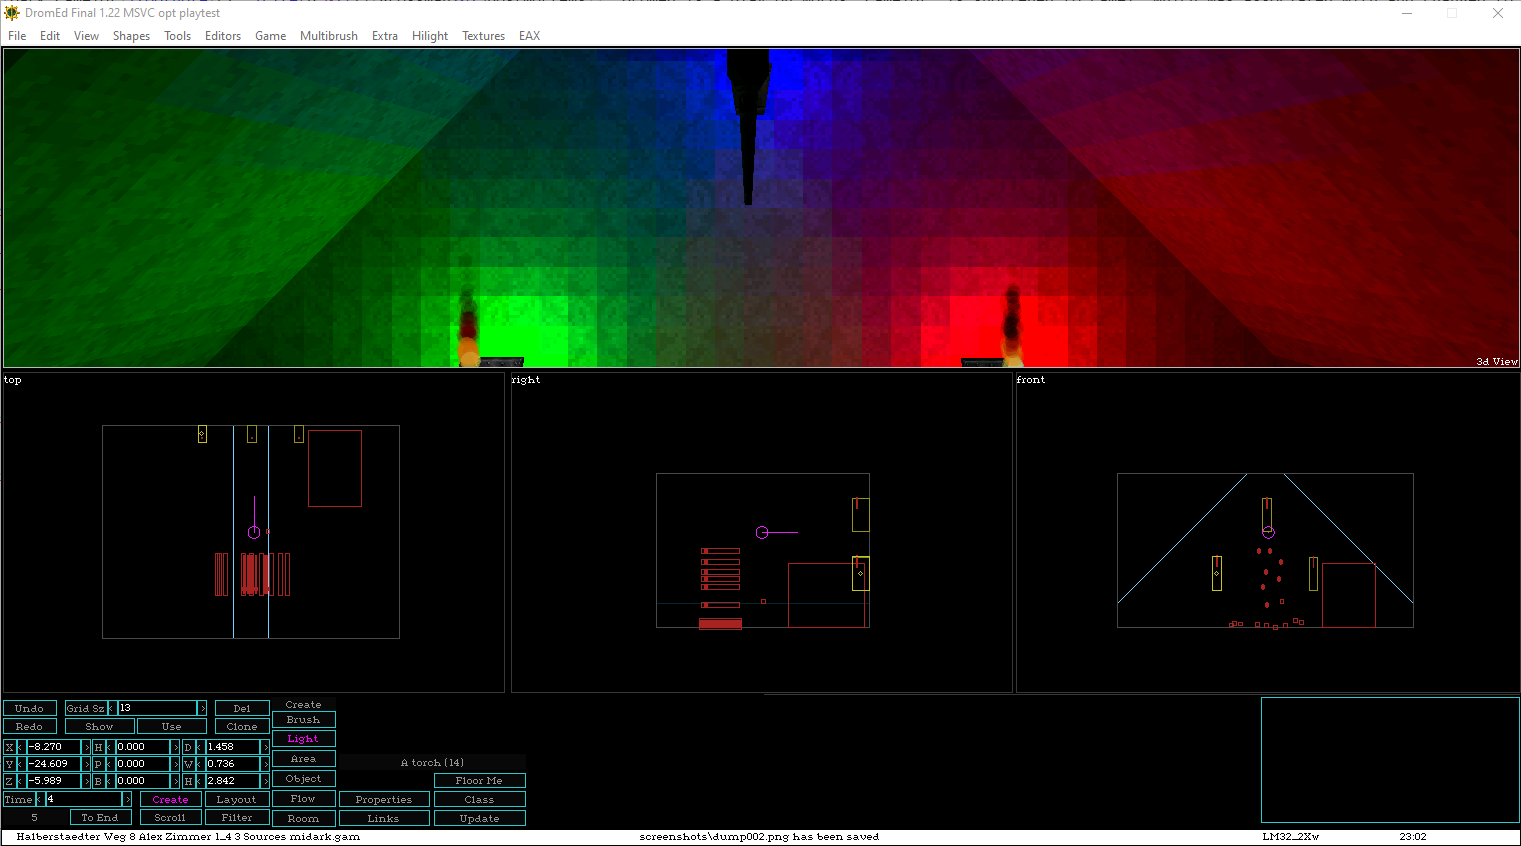
\includegraphics[width=1.00\textwidth]{img/PIX/Dromed_brushes.png}
	\caption[Overview of the Dromed editor]{Overview of the Dromed editor}
	\label{fig:DromedOverview}
\end{figure}

%\setcounter{figure}{0}  
\clearpage
\counterwithin{figure}{section}
\counterwithin{listing}{section}
\section{PIX overview} 

\begin{figure}[htbp]
	\centering
		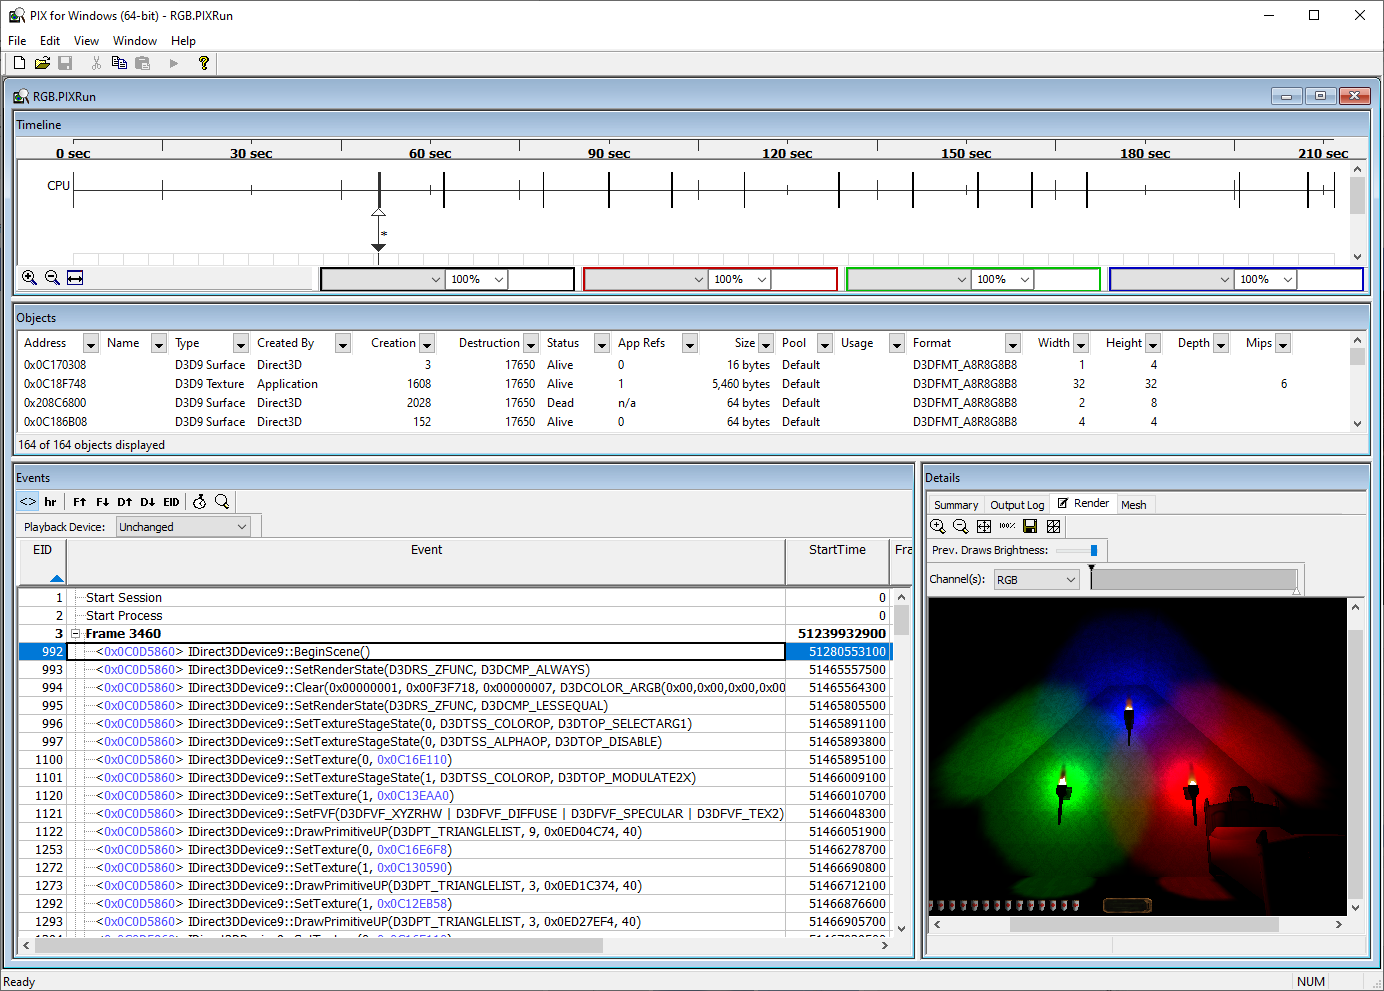
\includegraphics[width=1.00\textwidth]{img/PIX/PIX_overview.png}
	\caption[Overview of the PIX user interface]{Overview of the PIX user interface}
	\label{fig:PixOverview}
\end{figure}

%\setcounter{figure}{0}  
\clearpage
\counterwithin{figure}{section}
\counterwithin{listing}{section}
\section{Draw calls with lightmaps} 


\begin{figure}[htbp]
	\centering
		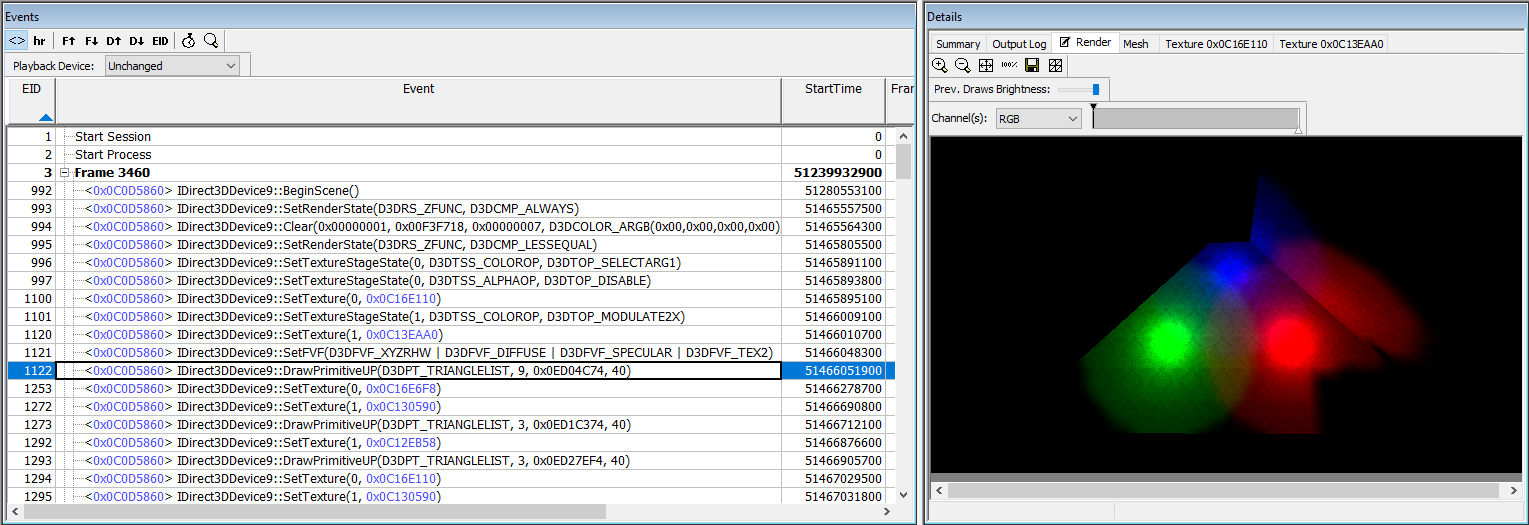
\includegraphics[width=1.00\textwidth]{img/PIX/PIX_first_frame_first_draw_call.png}
	\caption[First draw call of the first frame]{First draw call of the first frame}
	\label{fig:PixFirstFrameFirstDrawCall}
\end{figure}

\begin{listing}[htbp]
\begin{minted}[mathescape,
               linenos,
               numbersep=5pt,
							fontsize=\small,
							firstnumber=11,
               gobble=0,
               frame=lines,
               framesep=2mm]{C++}

BeginScene()
SetRenderState(D3DRS_ZFUNC, D3DCMP_ALWAYS)
Clear(0x00000001, 0x00F3F718, 0x00000007
      , D3DCOLOR_ARGB(0x00,0x00,0x00,0x00), 1.000f, 0x00000000)
SetRenderState(D3DRS_ZFUNC, D3DCMP_LESSEQUAL)
SetTextureStageState(0, D3DTSS_COLOROP, D3DTOP_SELECTARG1)
SetTextureStageState(0, D3DTSS_ALPHAOP, D3DTOP_DISABLE)
SetTexture(0, 0x0C16E110)
SetTextureStageState(1, D3DTSS_COLOROP, D3DTOP_MODULATE2X)
SetTexture(1, 0x0C13EAA0)
SetFVF(D3DFVF_XYZRHW | D3DFVF_DIFFUSE | D3DFVF_SPECULAR | D3DFVF_TEX2)
DrawPrimitiveUP(D3DPT_TRIANGLELIST, 9, 0x0ED04C74, 40)
SetTexture(0, 0x0C16E6F8)
SetTexture(1, 0x0C130590)
DrawPrimitiveUP(D3DPT_TRIANGLELIST, 3, 0x0ED1C374, 40)
\end{minted}
\caption[First draw call of the first frame]{First draw call of the first frame}
\label{lst:FirstFrameFirstDrawCalls}
\end{listing}




\begin{figure}[htbp]
	\centering
		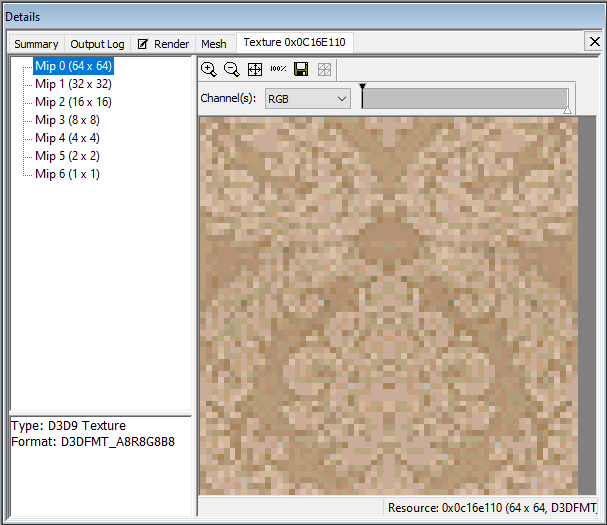
\includegraphics[width=1.00\textwidth]{img/PIX/PIX_wallpaper_details.png}
	\caption[Details of the wallpaper texture]{Details of the wallpaper texture}
	\label{fig:PIXWallpaperDetails}
\end{figure}


 
\begin{figure}[htbp]
	\centering
		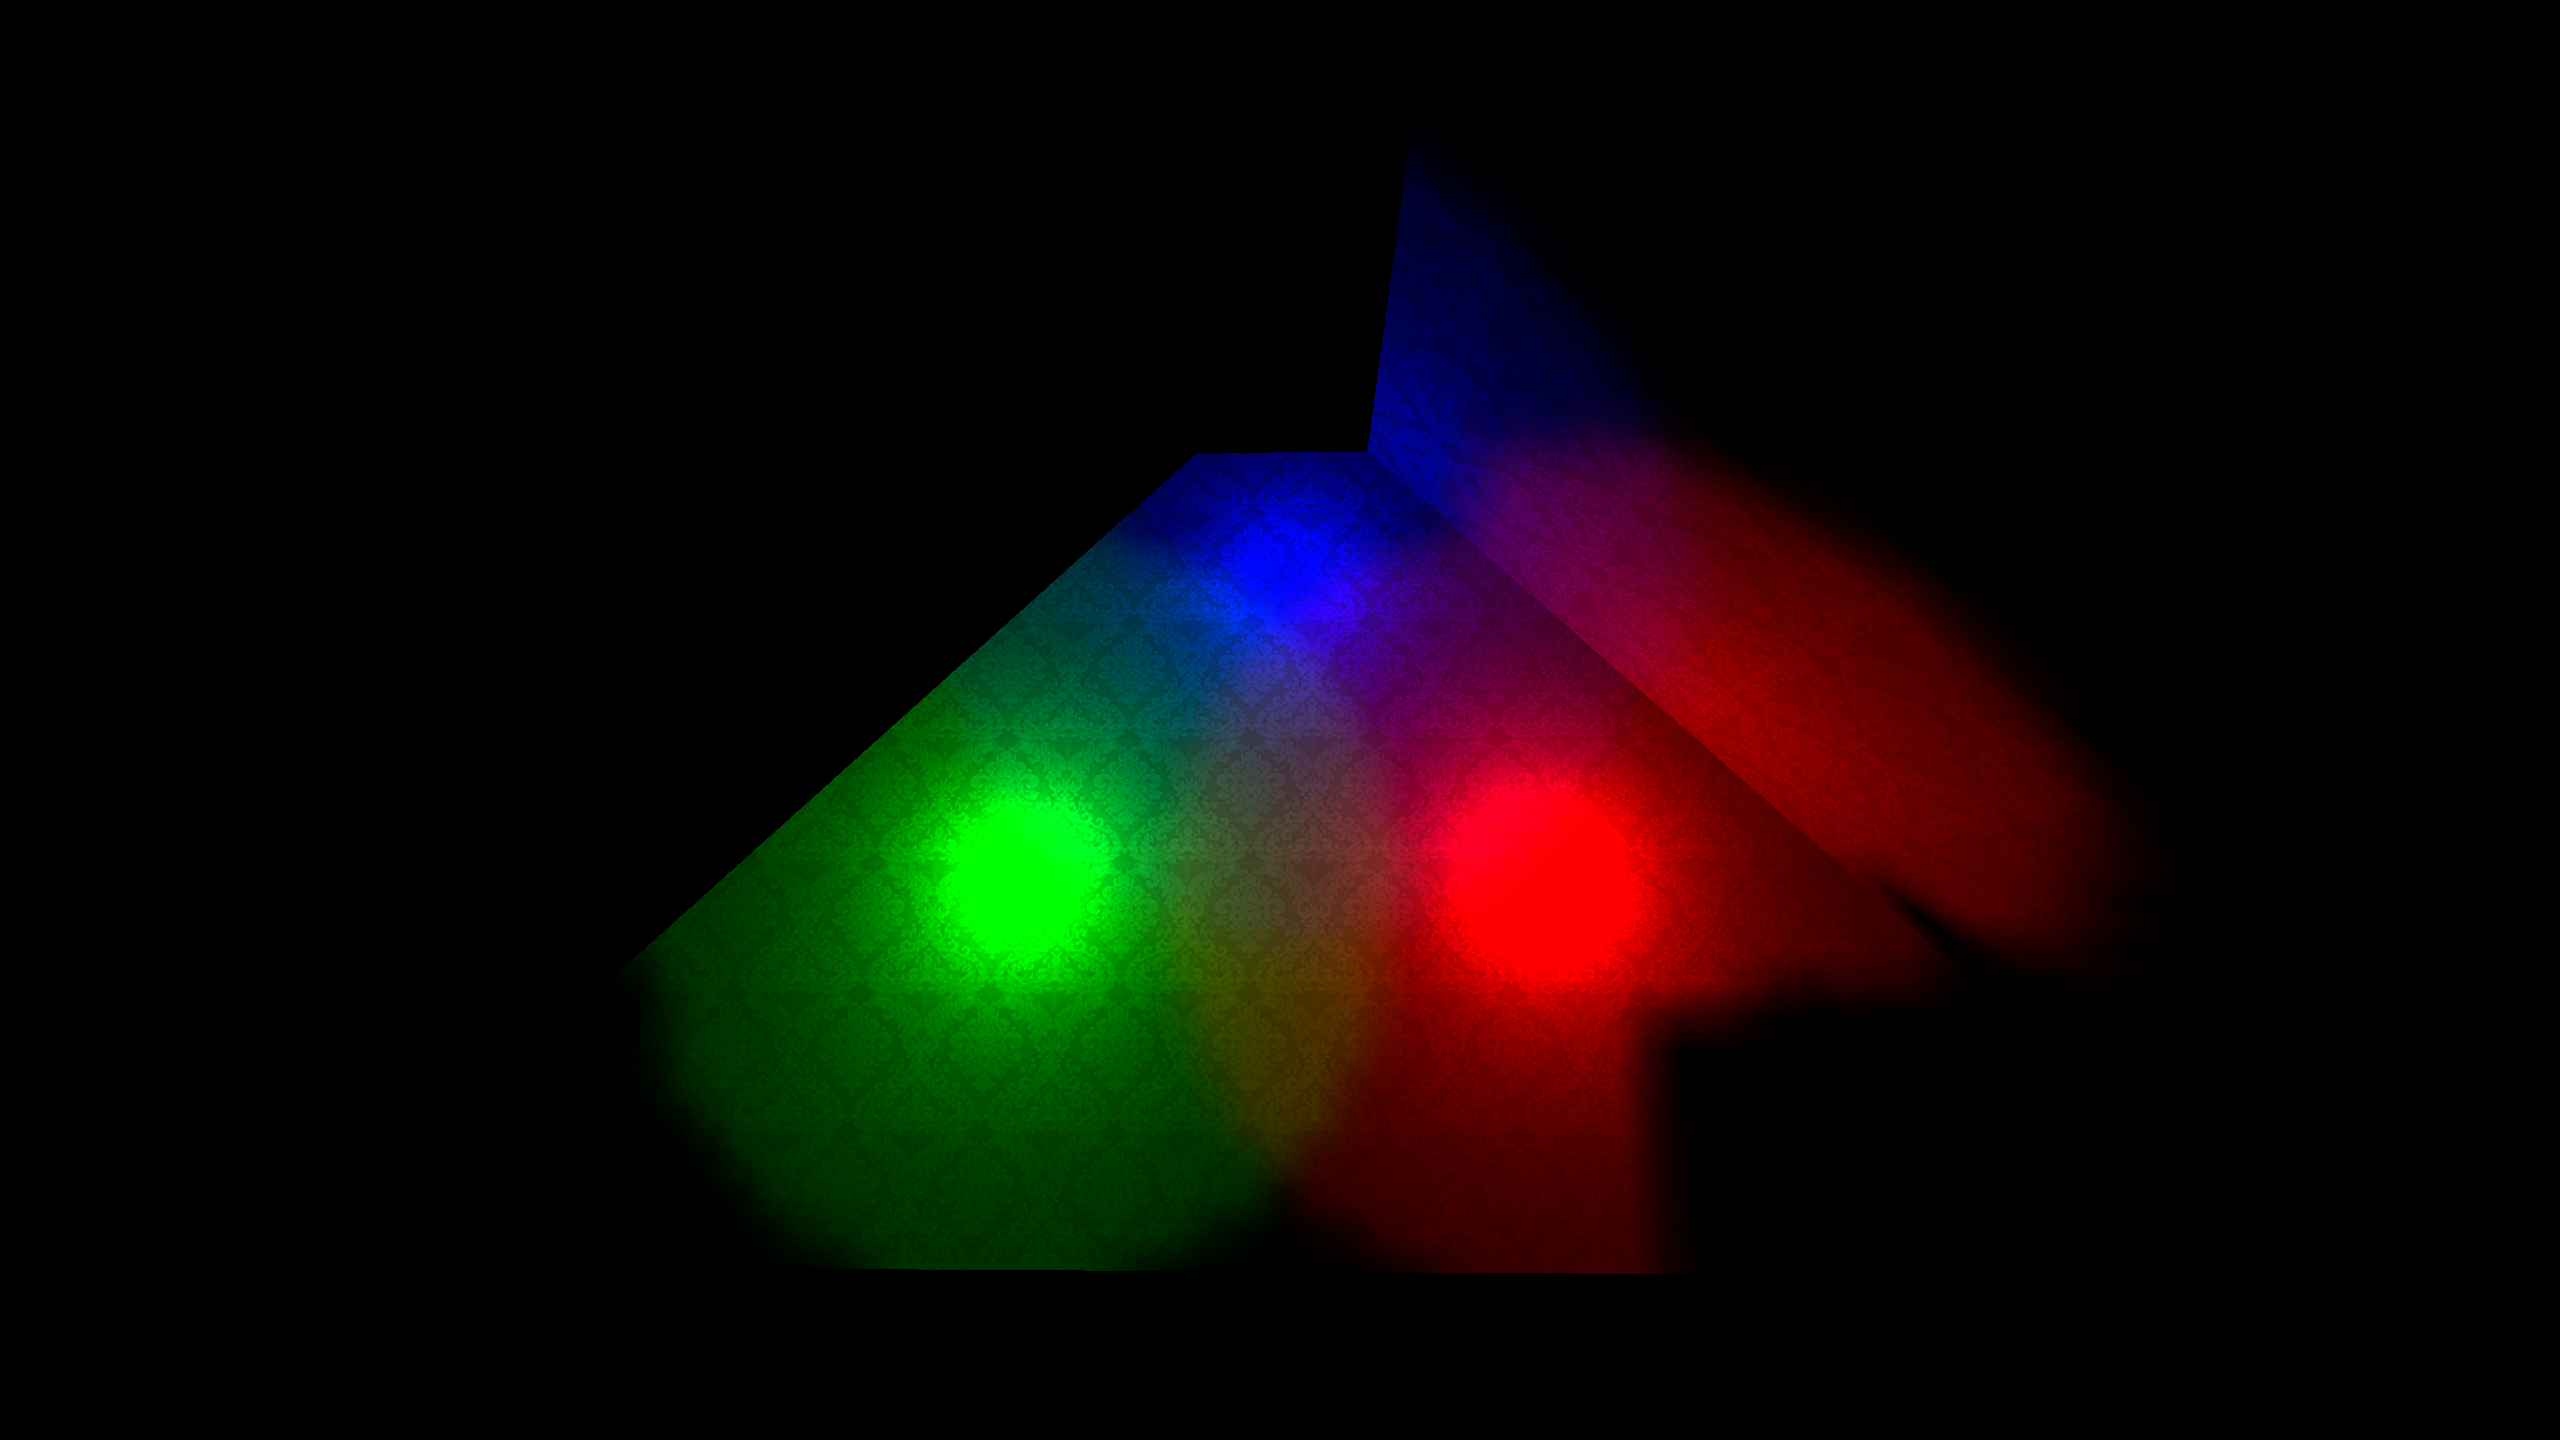
\includegraphics[width=1.00\textwidth]{img/PIX/PIX_lightbaking_render.png}
	\caption[Render of mesh with lightmap texture]{Render of mesh with lightmap texture}
	\label{fig:PIXLightmapRender}
\end{figure}

\begin{figure}[htbp]
	\centering
		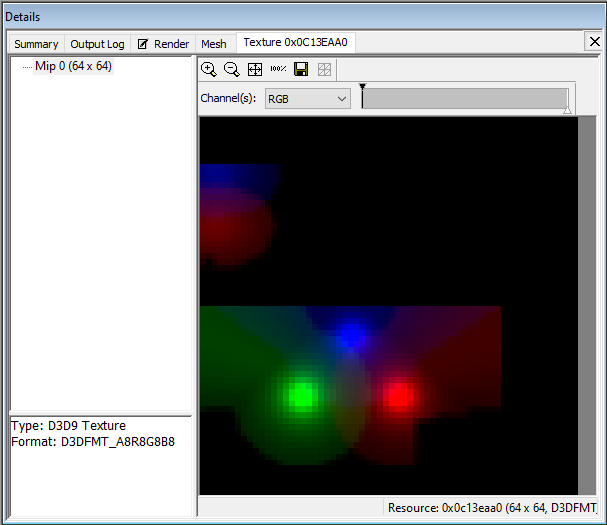
\includegraphics[width=1.00\textwidth]{img/PIX/PIX_lightmap_details.png}
	\caption[Details of the lightmap texture]{Details of the lightmap texture}
	\label{fig:PIXLightmapDetails}
\end{figure}

\begin{figure}[htbp]
	\centering
		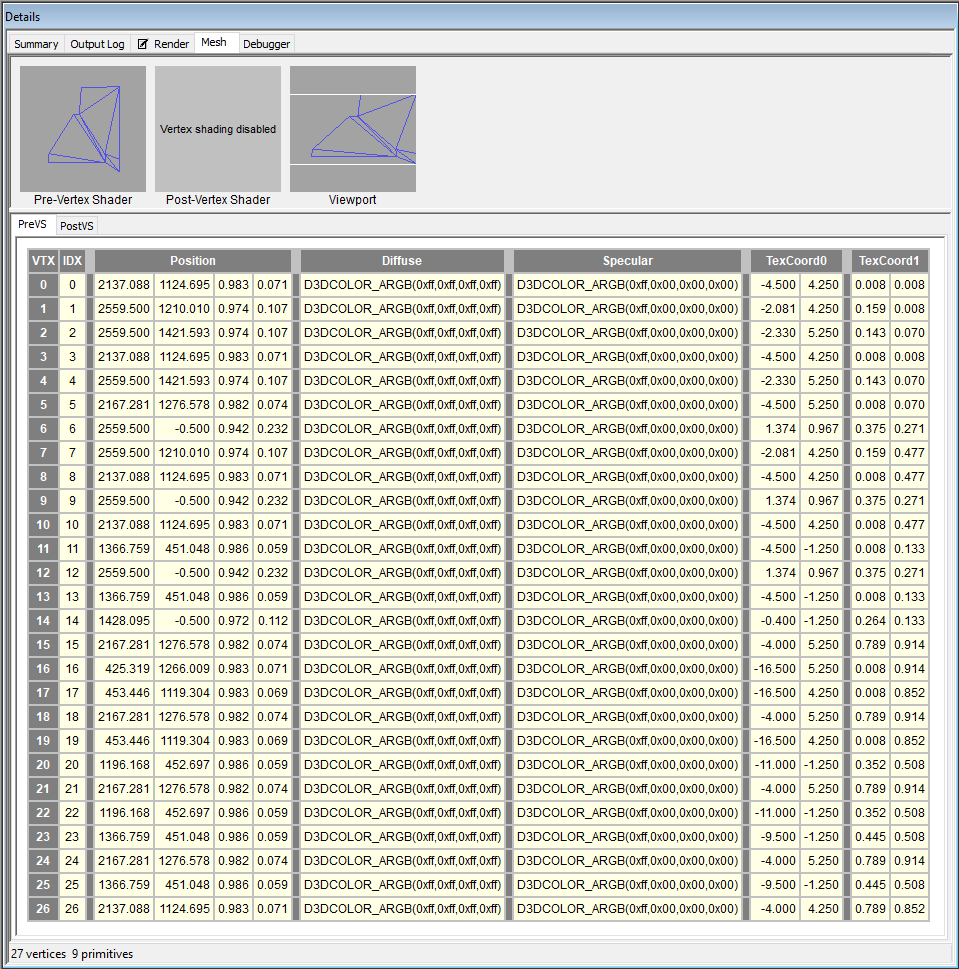
\includegraphics[width=1.00\textwidth]{img/PIX/PIX_lightbaking_details.png}
	\caption[Details of mesh with lightmap texture]{Details of mesh with lightmap texture}
	\label{fig:PIXLightmapMeshDetails}
\end{figure}

%\setcounter{figure}{0}  
\clearpage
\counterwithin{figure}{section}
\counterwithin{listing}{section}
\section{Draw calls with vertex lighting}

\begin{listing}[htbp]
\begin{minted}[mathescape,
               linenos,
               numbersep=5pt,
							fontsize=\small,
							firstnumber=11,
               gobble=0,
               frame=lines,
               framesep=2mm]{C++}
SetTextureStageState(0, D3DTSS_COLOROP, D3DTOP_MODULATE) 
SetTextureStageState(0, D3DTSS_ALPHAOP, D3DTOP_MODULATE)	
SetTextureStageState(1, D3DTSS_COLOROP, D3DTOP_DISABLE)				
SetTexture(0, 0x0C16E3B0)	
SetTexture(1, NULL)			
SetTexture(0, 0x0C16E8F0)	
SetFVF(D3DFVF_XYZRHW | D3DFVF_DIFFUSE | D3DFVF_SPECULAR | D3DFVF_TEX1)		
DrawPrimitiveUP(D3DPT_TRIANGLELIST, 8, 0x0ED1C374, 32)	
\end{minted}
\caption[Draw calls for the first vertex lit mesh]{Draw calls for the first vertex lit mesh}
\label{lst:DrawCallsForTheFirstVertexLitMesh}
\end{listing}

\begin{figure}[htbp]
	\centering
		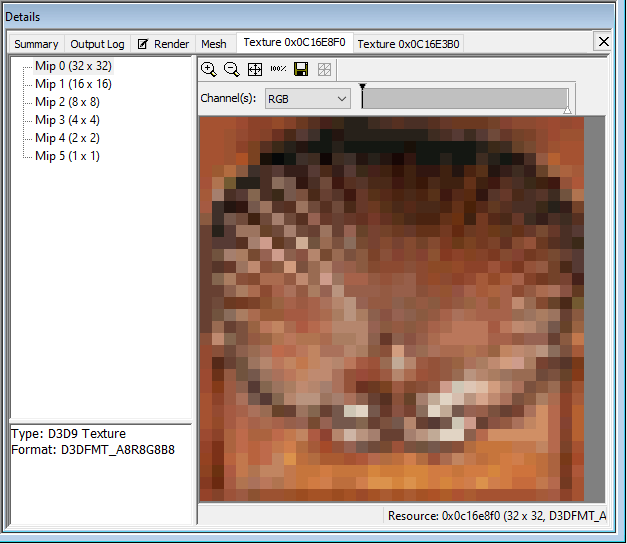
\includegraphics[width=1.00\textwidth]{img/PIX/PIX_bedend_details.png}
	\caption[Bed headboard texture]{Bed headboard texture}
	\label{fig:BedHeadboardTexture}
\end{figure}

\clearpage

\begin{figure}[htbp]
	\centering
		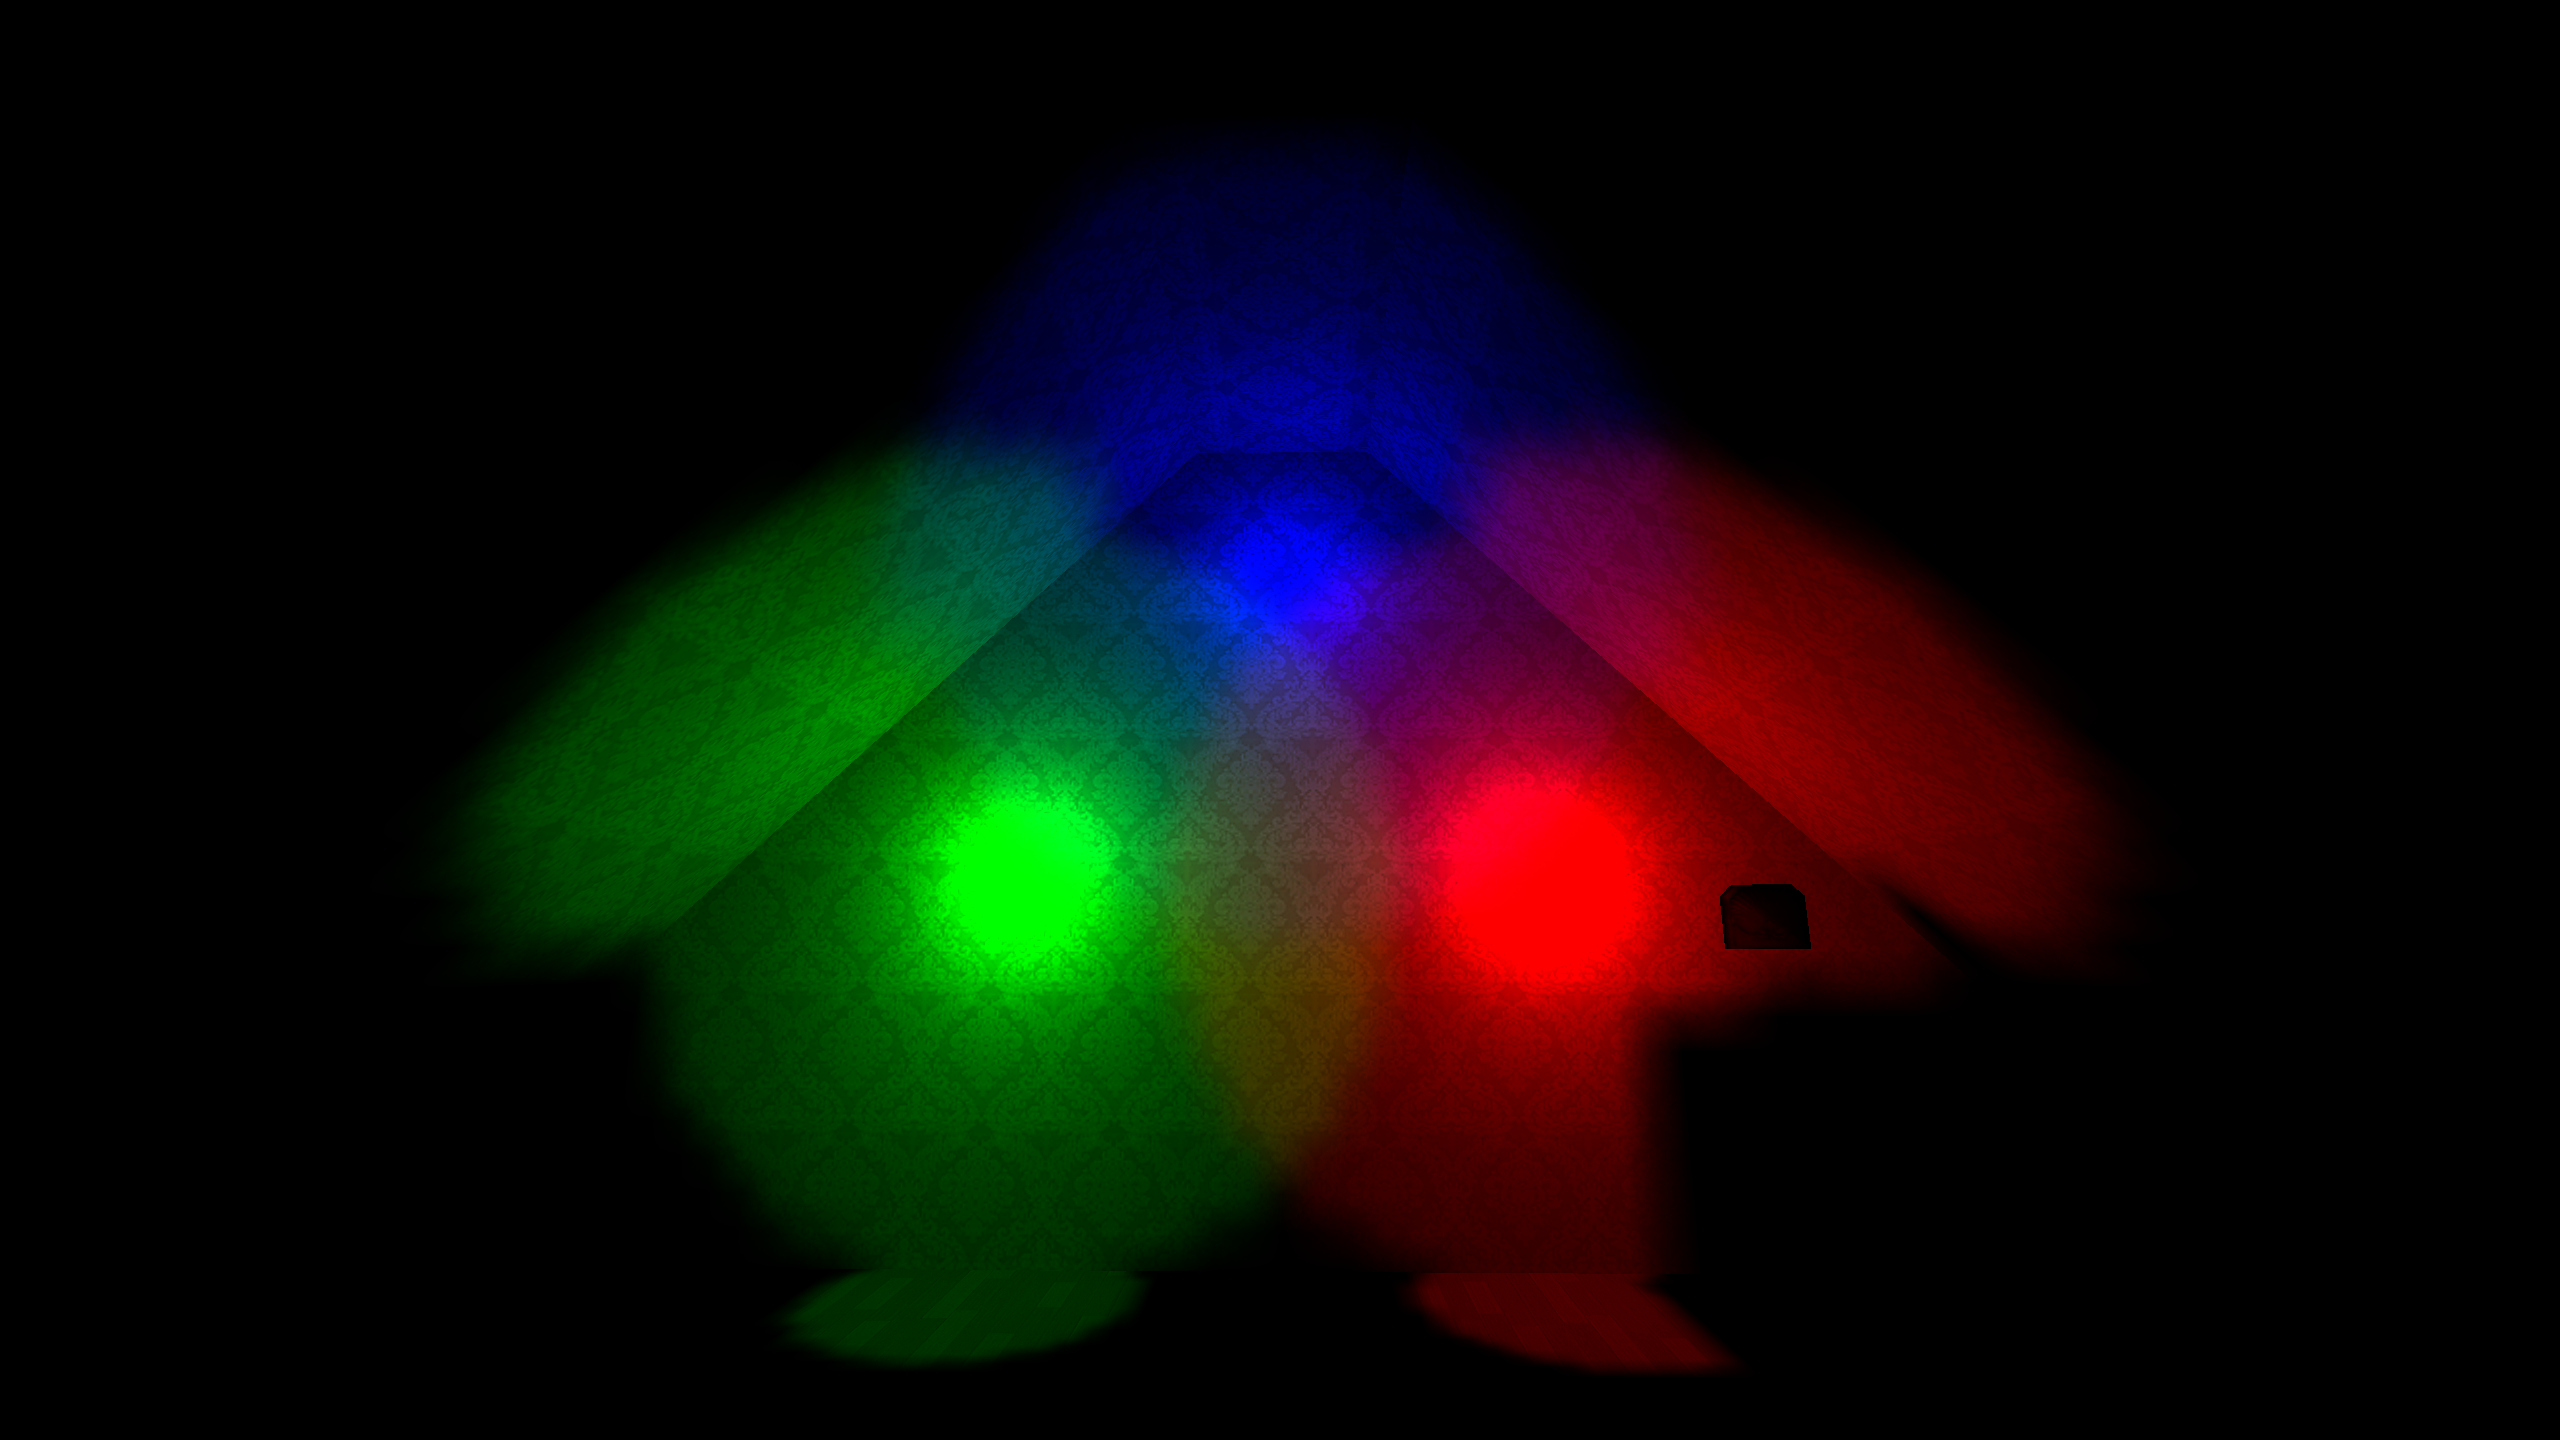
\includegraphics[width=1.00\textwidth]{img/PIX/vertex_lit_mesh_render.png}
	\caption[Render of the first mesh with vertex lighting]{Render of the first mesh with vertex lighting}
	\label{fig:RenderForFirstVertexLitMesh}
\end{figure}



\begin{figure}[htbp]
	\centering
		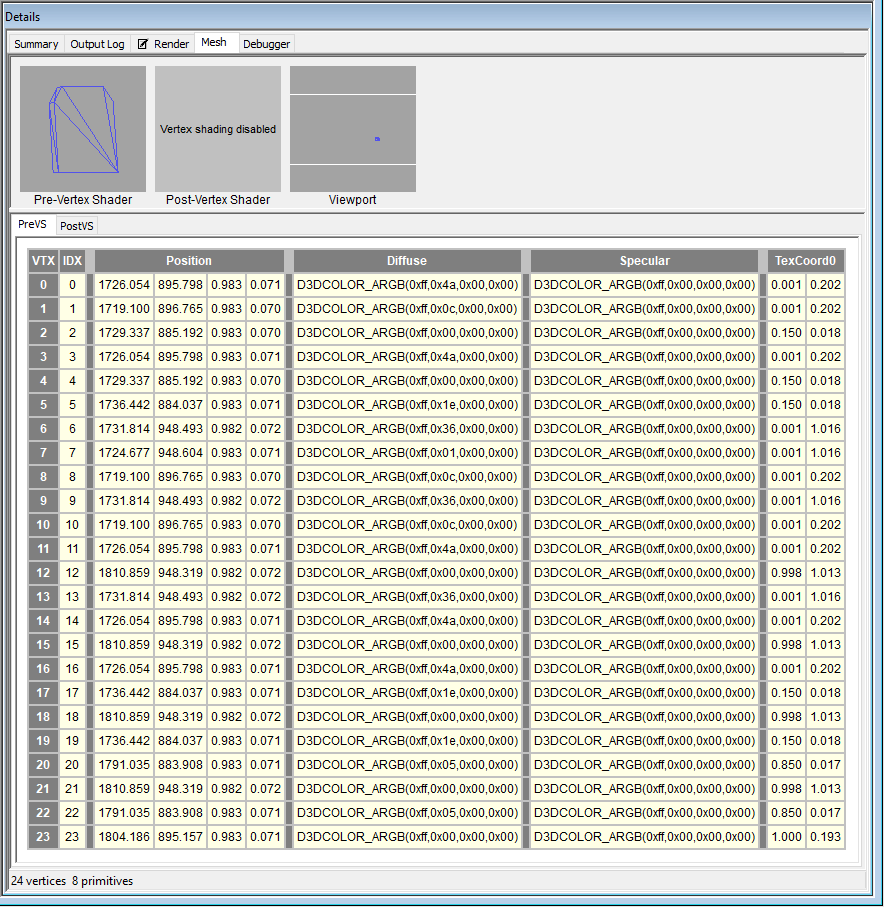
\includegraphics[width=1.00\textwidth]{img/PIX/vertex_lit_mesh_details.png}
	\caption[Details of the first mesh with vertex lighting]{Details of the first mesh with vertex lighting}
	\label{fig:DetailsForFirstVertexLitMesh}
\end{figure}



 


%\setcounter{figure}{0}  
\clearpage
\label{lab:RenderedFramesAndLightmaps}
\counterwithin{figure}{section}
\counterwithin{listing}{section}
\section{Lightmap and render - reg, green and blue torches lit} 
\label{lab:RGB}

\begin{figure}[htbp]
	\centering
		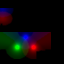
\includegraphics[width=0.40\textwidth]{img/PIX/rgb.png}
	\caption[Lightmap of scene with all torches lit]{Lightmap of scene with all torches lit}
	\label{fig:LightmapRGB}
\end{figure}
\begin{figure}[htbp]
	\centering
		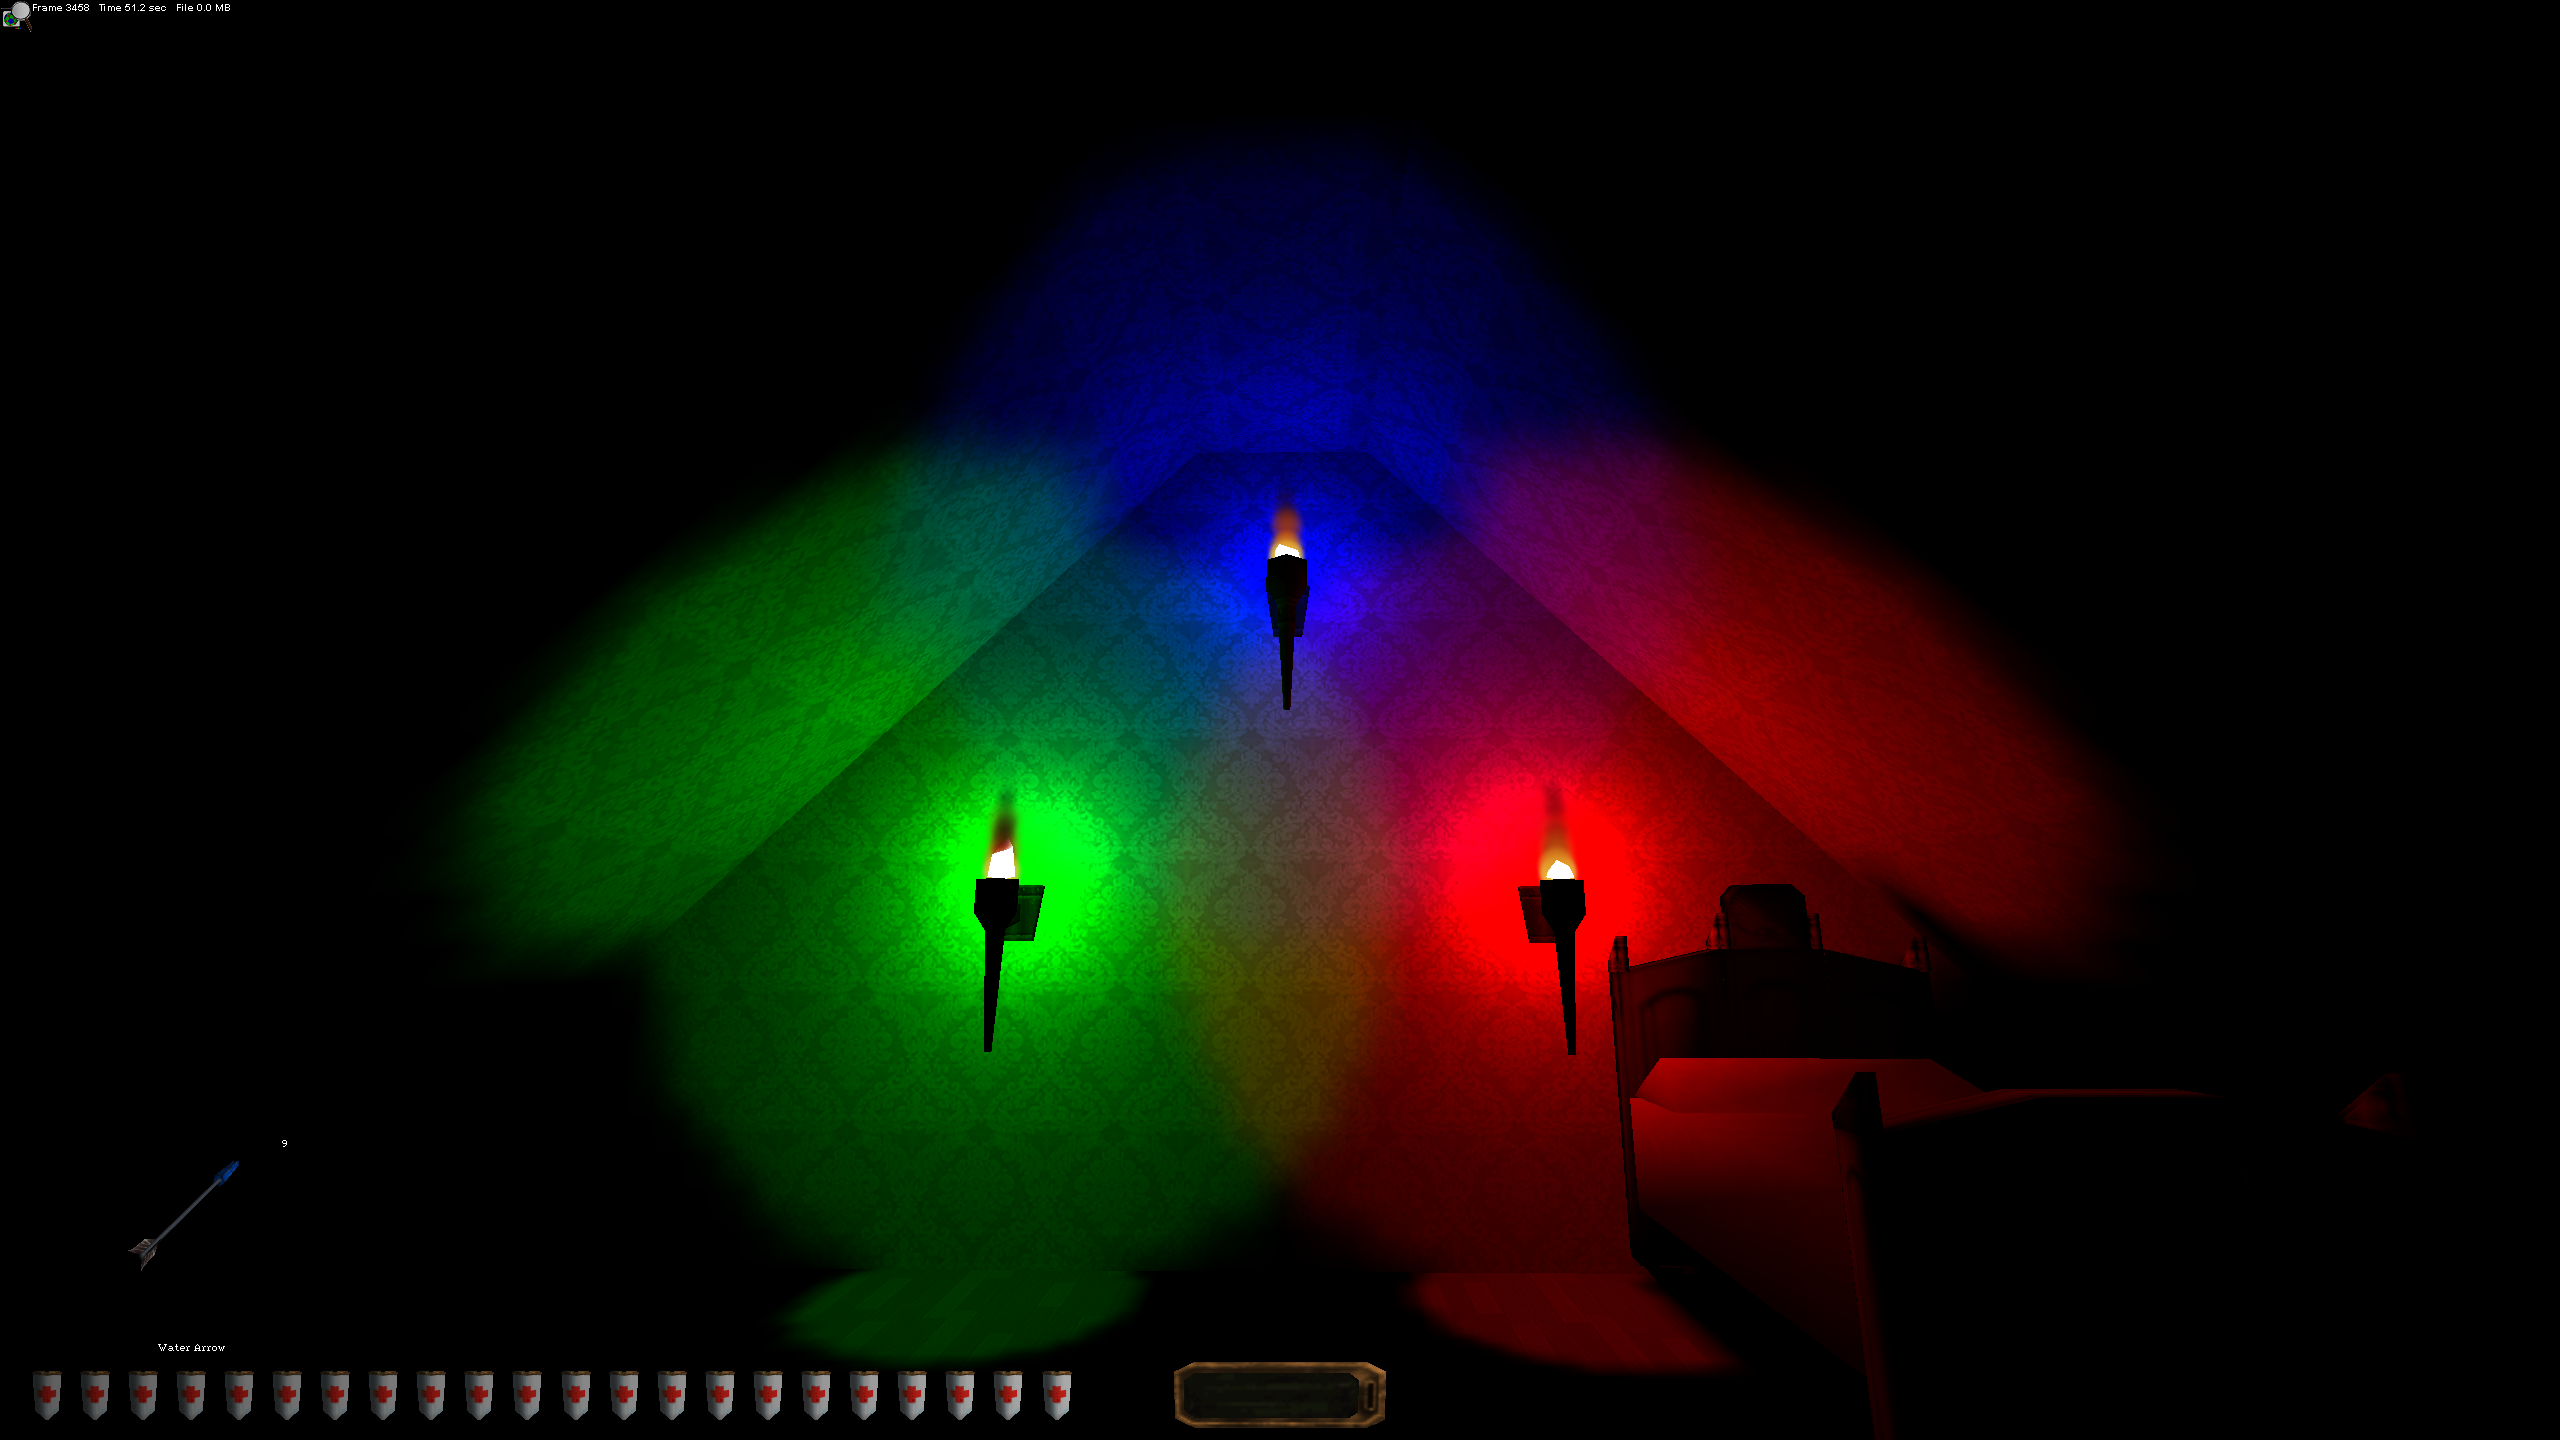
\includegraphics[width=1.00\textwidth]{img/PIX/render_rgb.png}
	\caption[Render of scene with all torches lit]{Render of scene with all torches lit}
	\label{fig:RenderRGB}
\end{figure}

%\setcounter{figure}{0}  
\clearpage
\counterwithin{figure}{section}
\counterwithin{listing}{section}
\section{Lightmap and render - red and green torches lit} 


\begin{figure}[htbp]
	\centering
		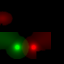
\includegraphics[width=0.40\textwidth]{img/PIX/rg.png}
	\caption[Lightmap of scene with red and green torches lit]{Lightmap of scene with red and green torches lit}
	\label{fig:LightmapRG}
\end{figure}
\begin{figure}[htbp]
	\centering
		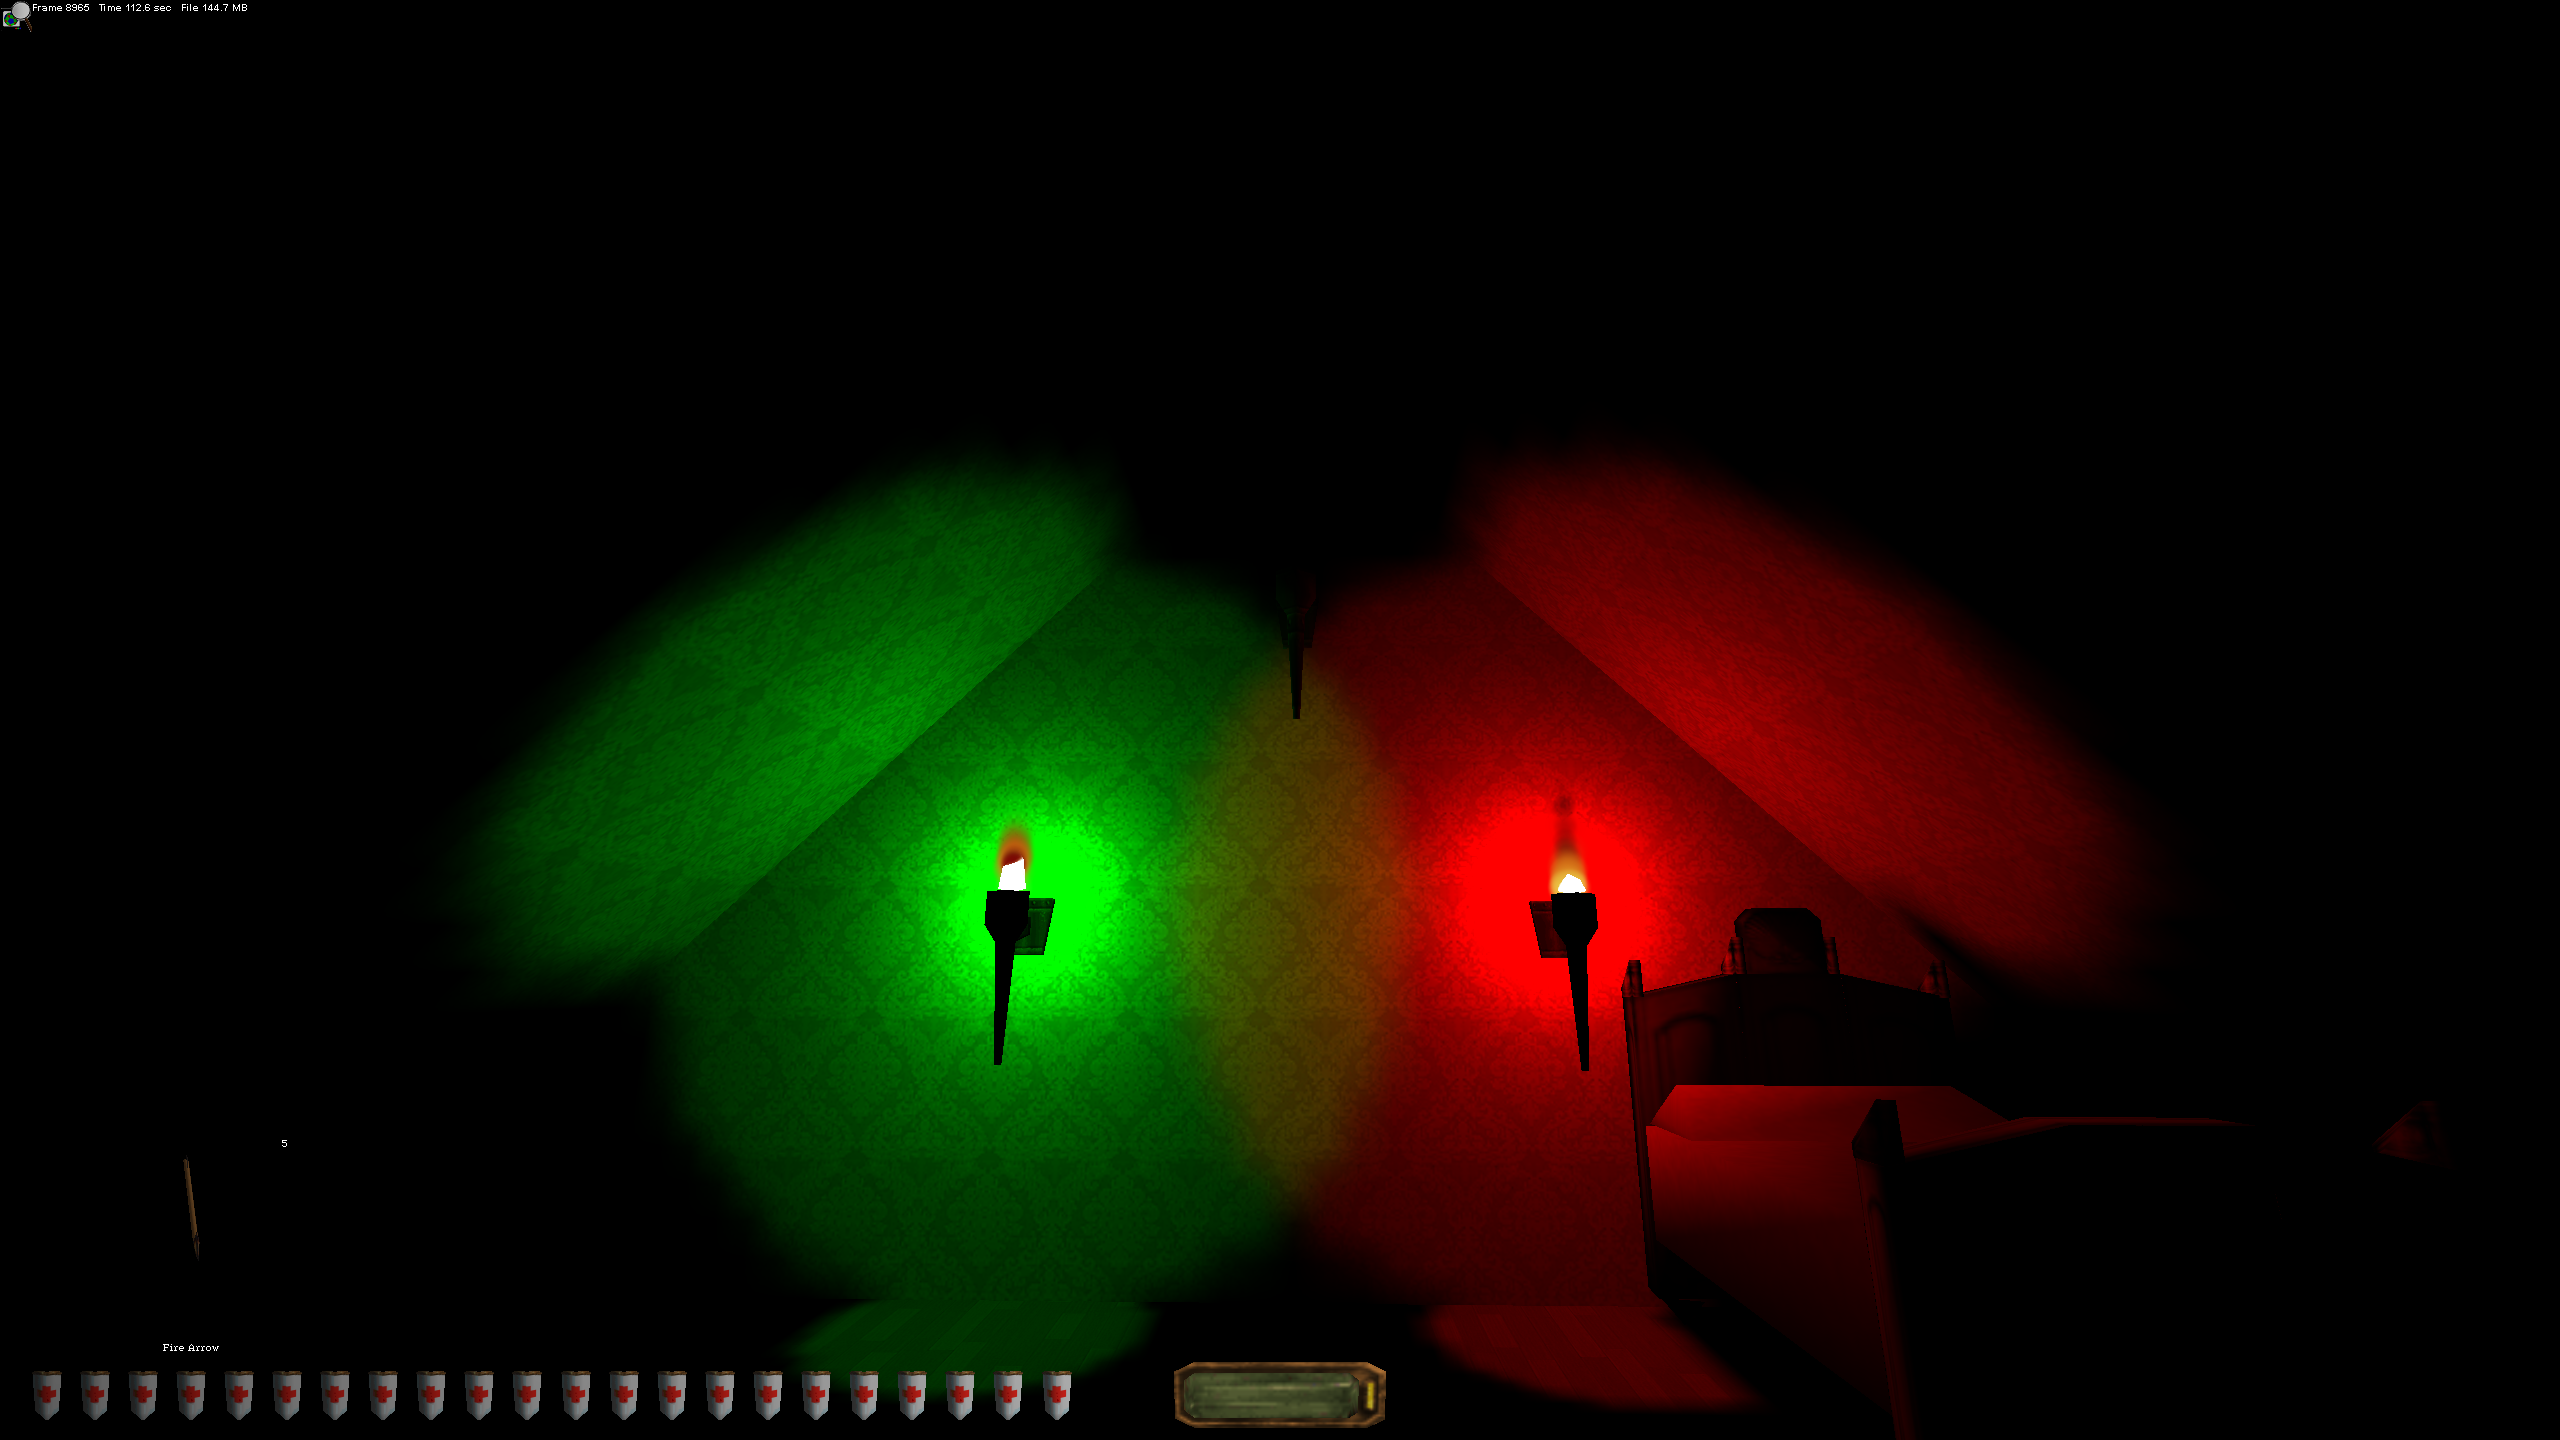
\includegraphics[width=1.00\textwidth]{img/PIX/render_rg.png}
	\caption[Render of scene with red and green torches lit]{Render of scene with red and green torches lit}
	\label{fig:RenderRG}
\end{figure}

%\setcounter{figure}{0}  
\clearpage
\counterwithin{figure}{section}
\counterwithin{listing}{section}
\section{Lightmap and render - red and blue torches lit} 


\begin{figure}[htbp]
	\centering
		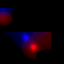
\includegraphics[width=0.40\textwidth]{img/PIX/rb.png}
	\caption[Lightmap of scene with red and blue torches lit]{Lightmap of scene with red and blue torches lit}
	\label{fig:LightmapRB}
\end{figure}
\begin{figure}[htbp]
	\centering
		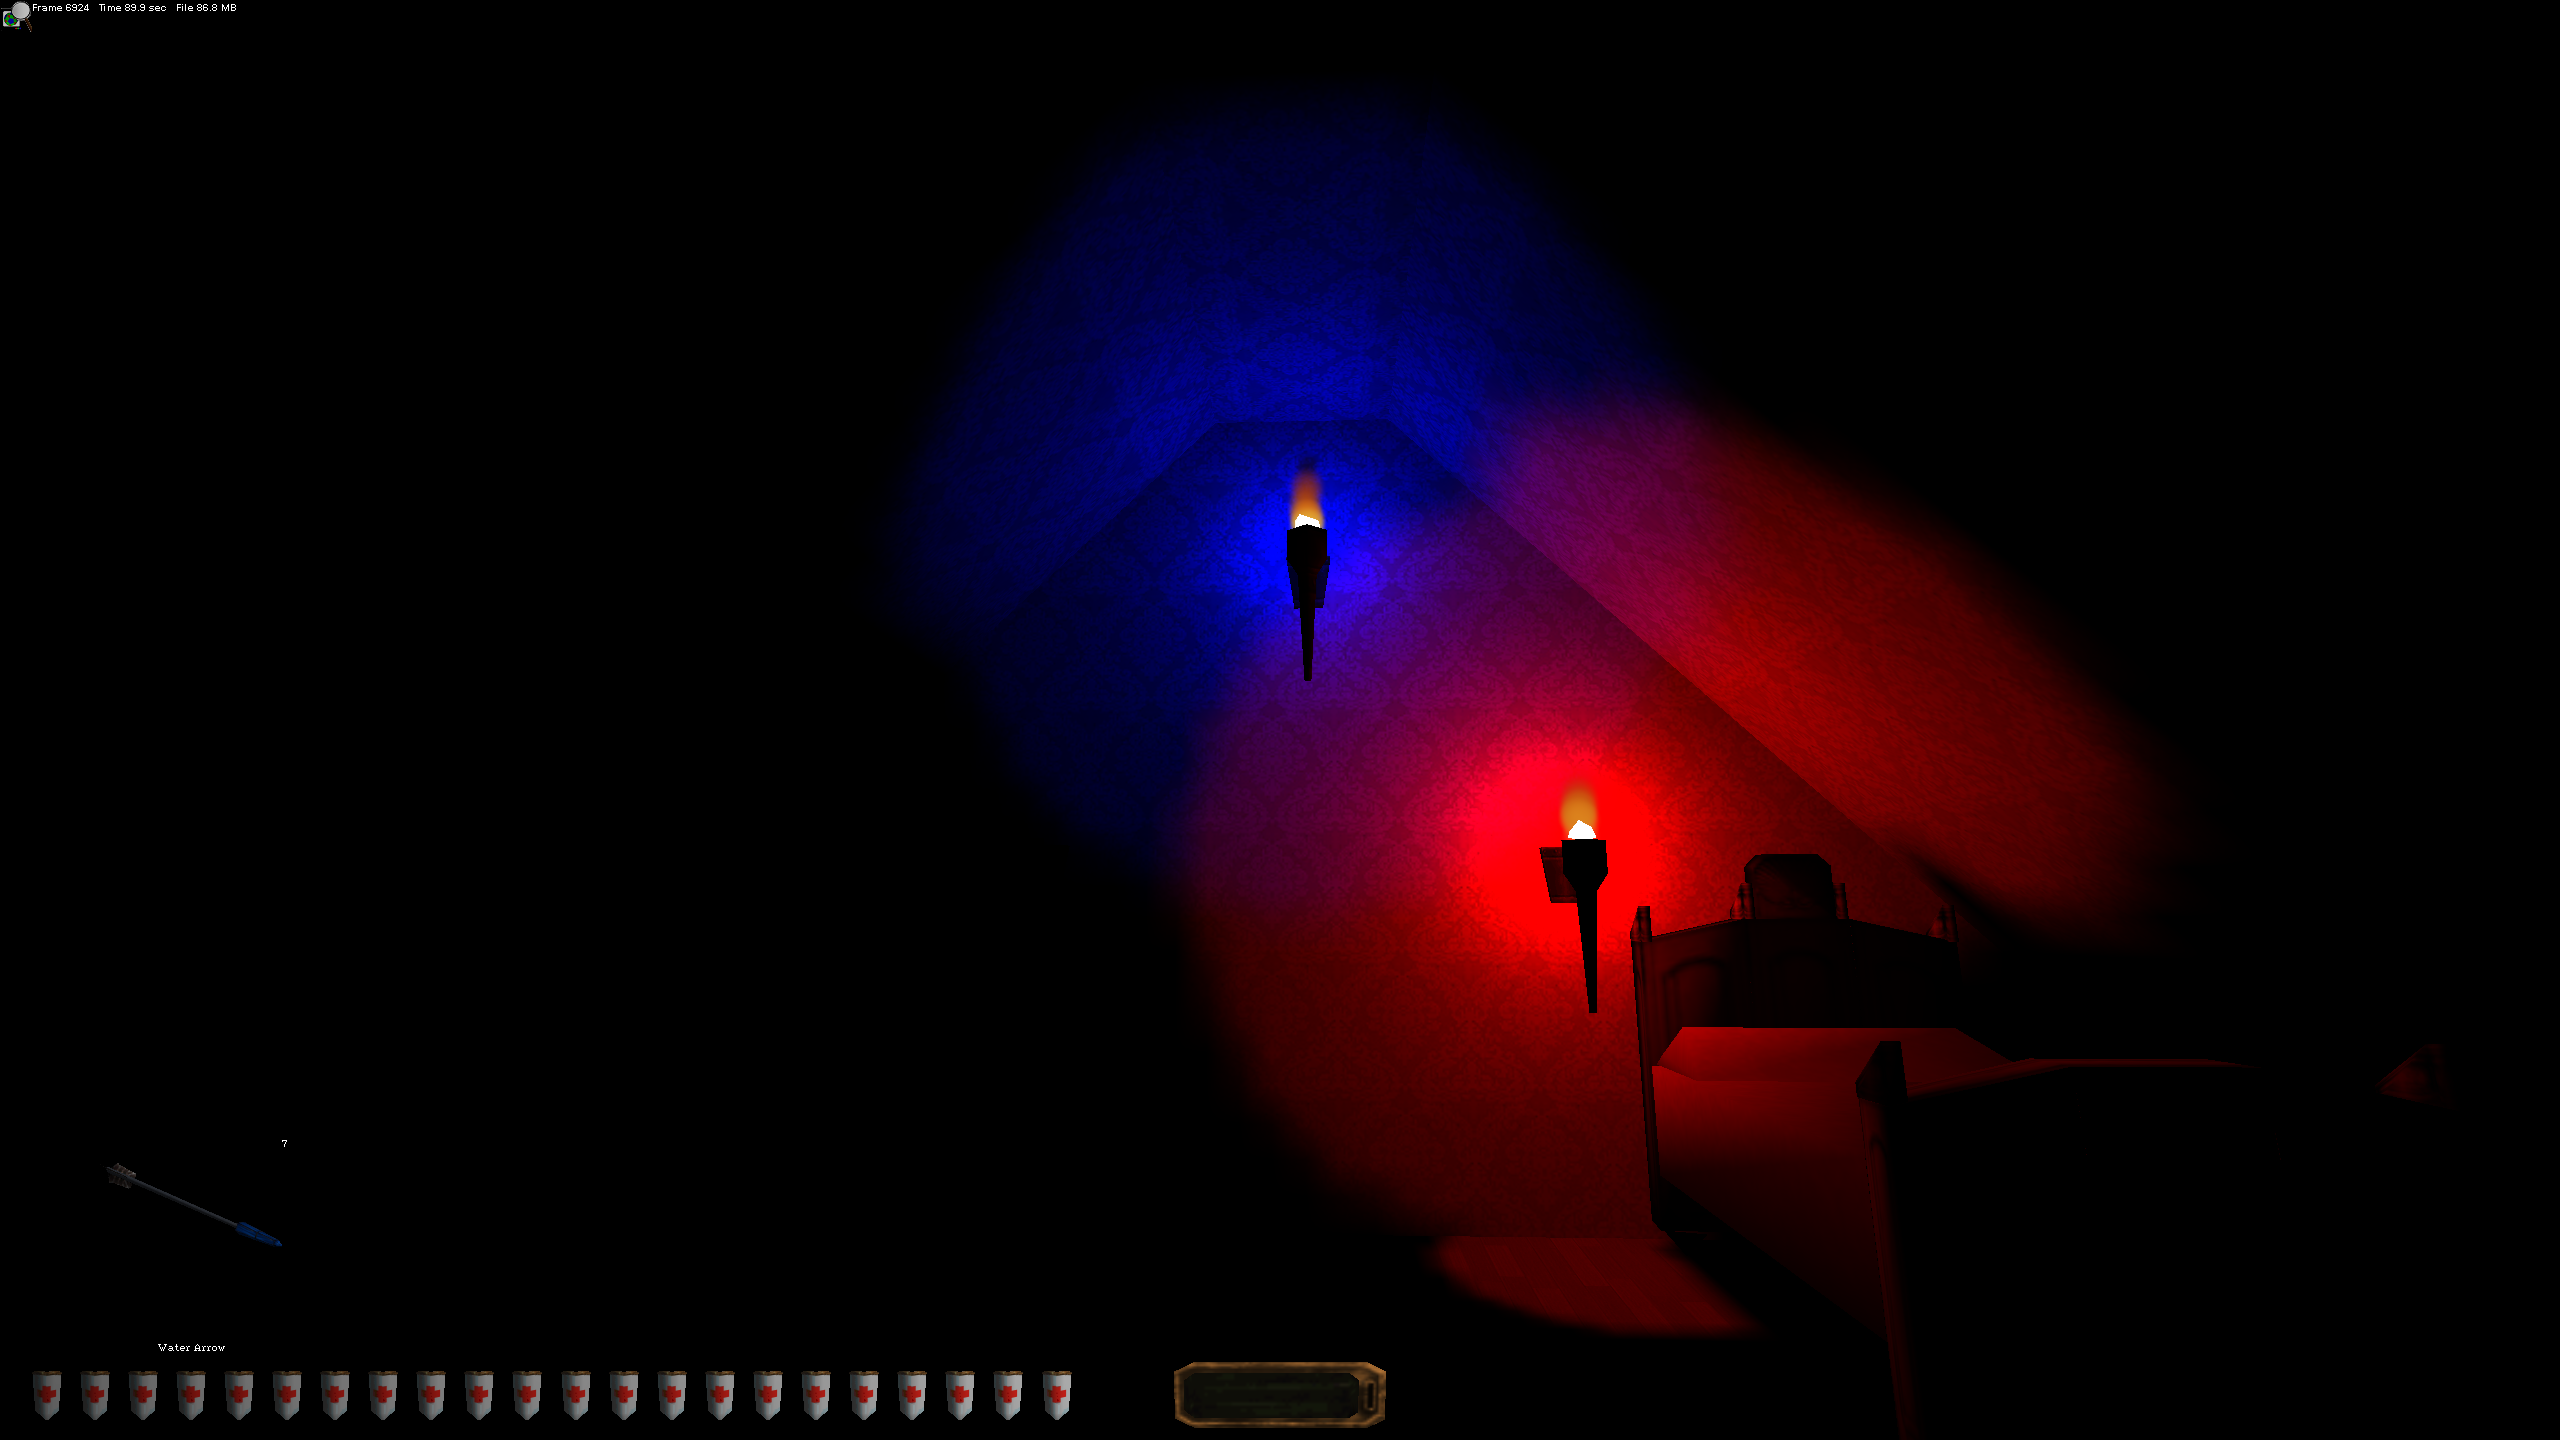
\includegraphics[width=1.00\textwidth]{img/PIX/render_rb.png}
	\caption[Render of scene with red and blue torches lit]{Render of scene with red and blue torches lit}
	\label{fig:RenderRB}
\end{figure}

%\setcounter{figure}{0}  
\clearpage
\counterwithin{figure}{section}
\counterwithin{listing}{section}
\section{Lightmap and render - green and blue torches lit} 


\begin{figure}[htbp]
	\centering
		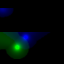
\includegraphics[width=0.40\textwidth]{img/PIX/gb.png}
	\caption[Lightmap of scene with green and blue torches lit]{Lightmap of scene with green and blue torches lit}
	\label{fig:LightmapGB}
\end{figure}
\begin{figure}[htbp]
	\centering
		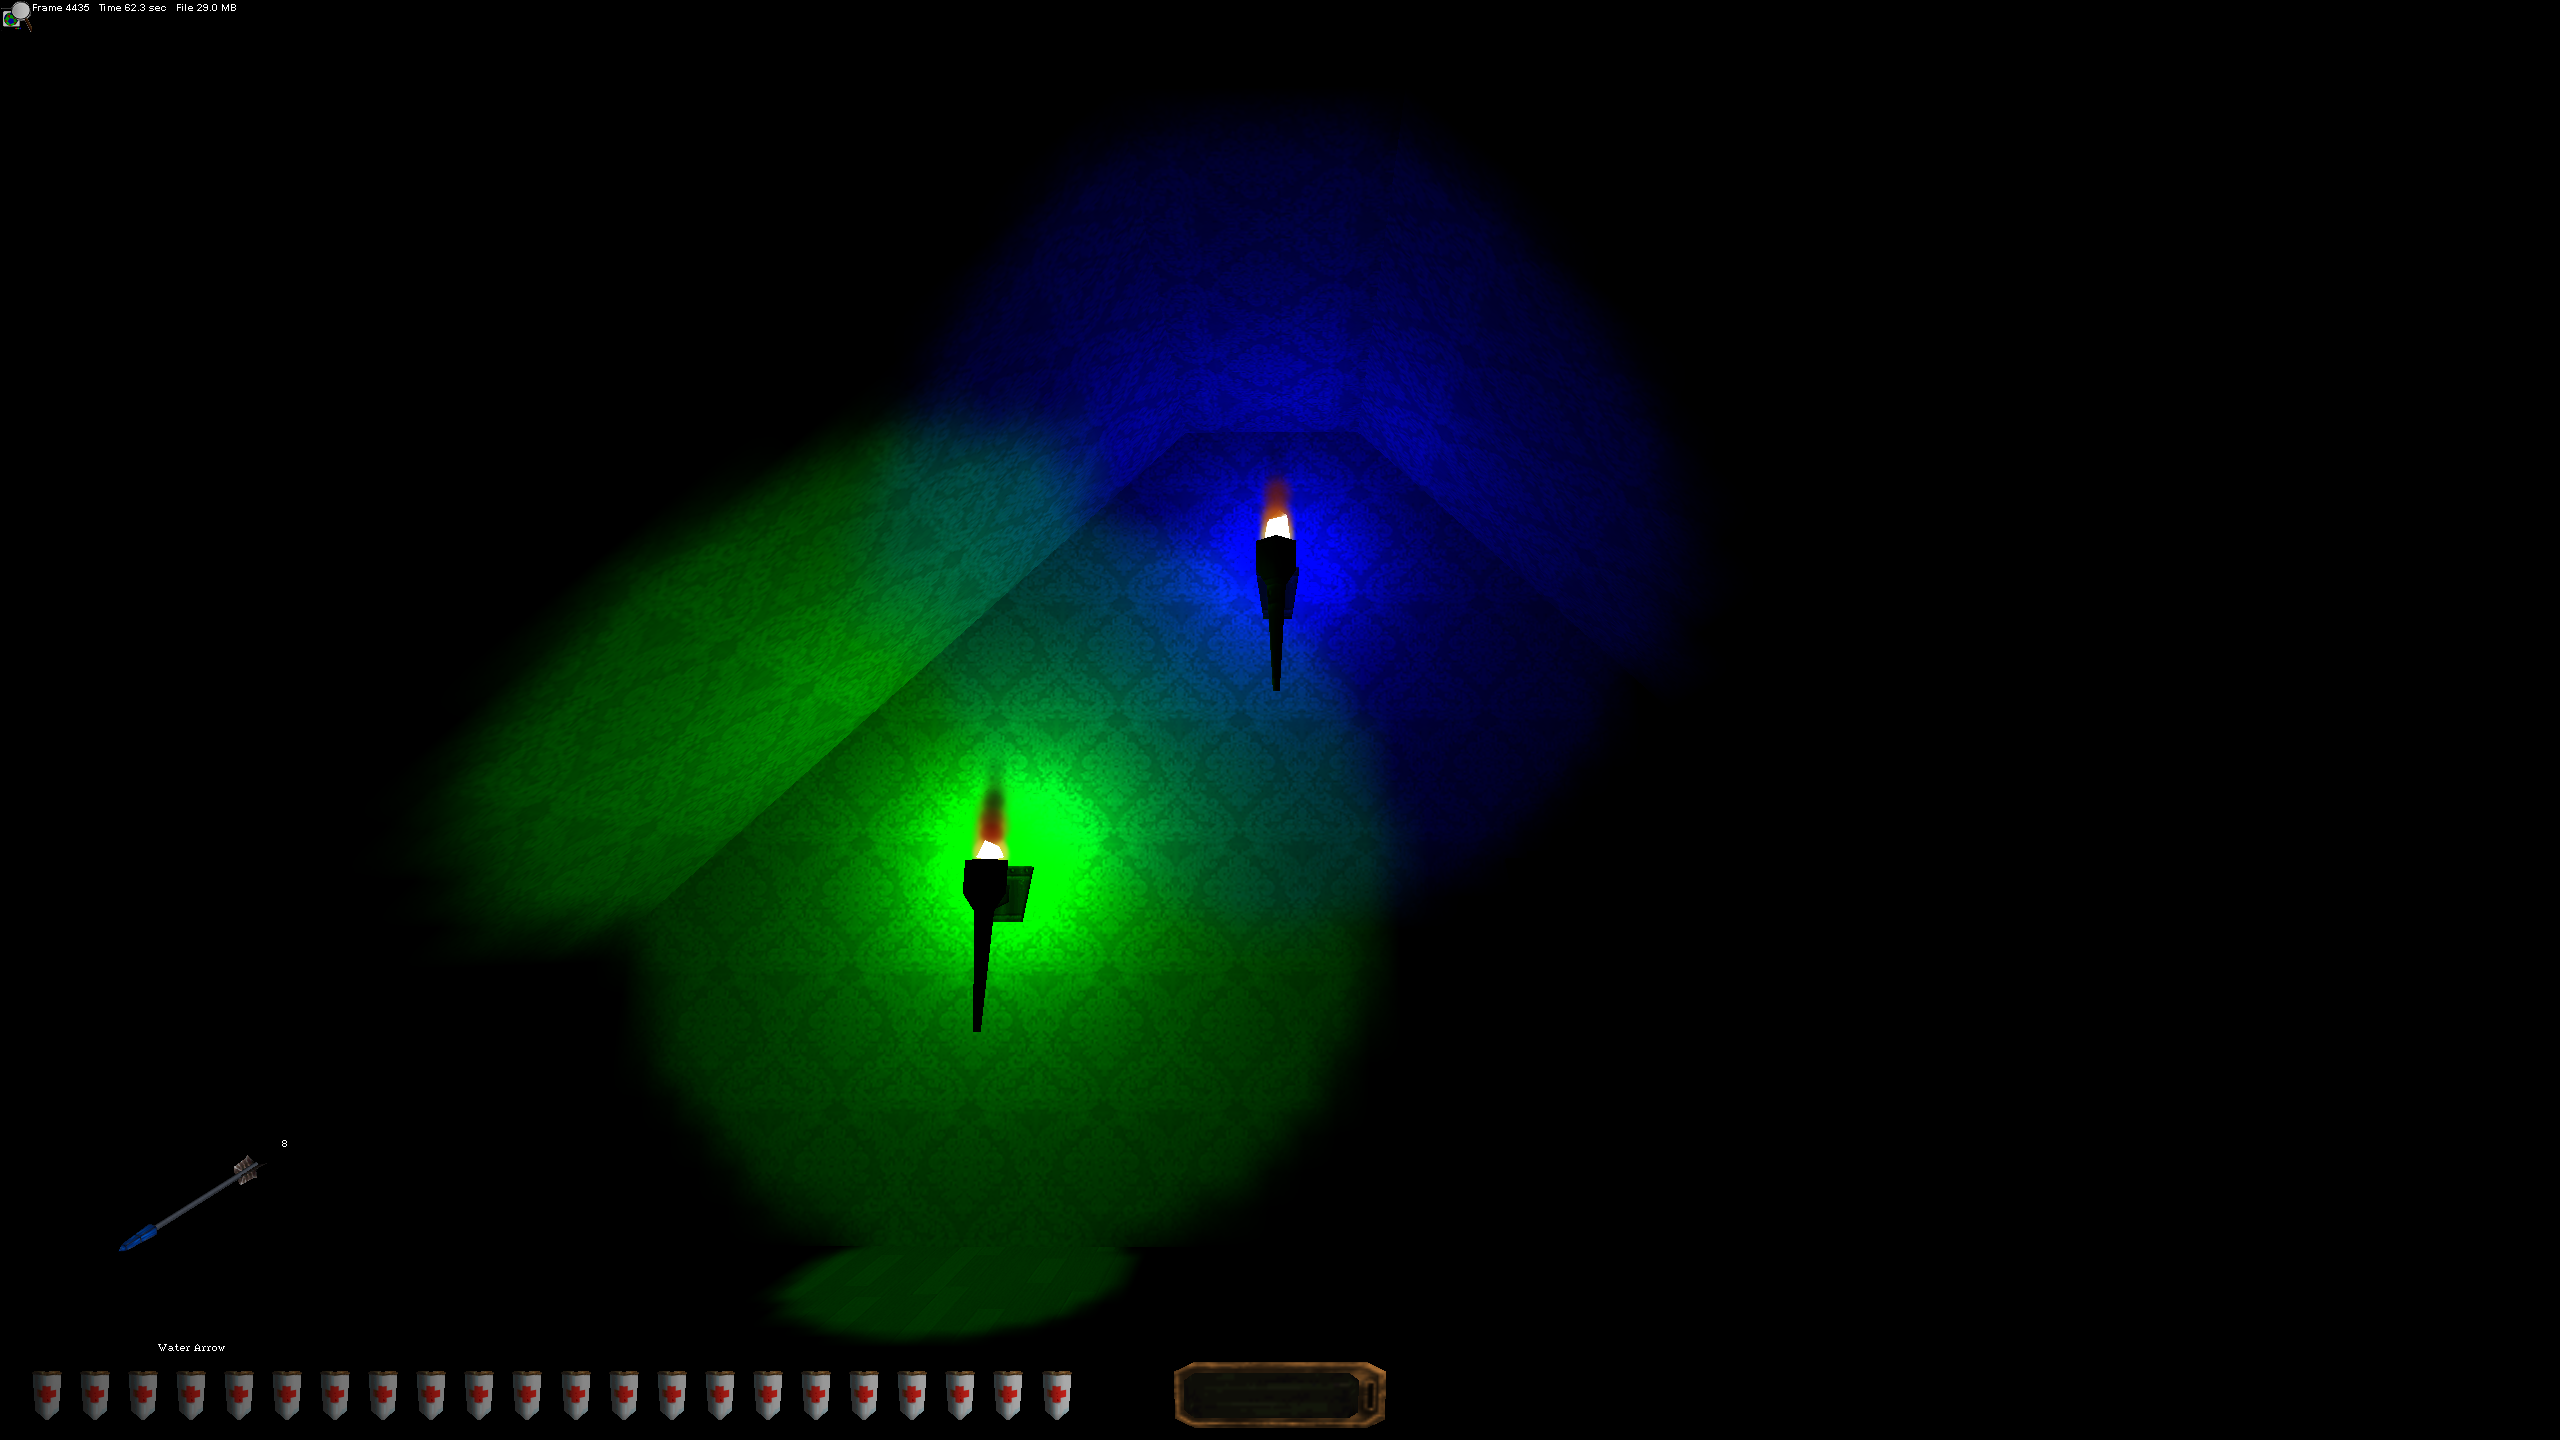
\includegraphics[width=1.00\textwidth]{img/PIX/render_gb.png}
	\caption[Render of scene with green and blue torches lit]{Render of scene with green and blue torches lit}
	\label{fig:RenderGB}
\end{figure}

%\setcounter{figure}{0}  
\clearpage
\counterwithin{figure}{section}
\counterwithin{listing}{section}
\section{Lightmap and render - red torch lit} 


\begin{figure}[htbp]
	\centering
		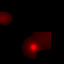
\includegraphics[width=0.40\textwidth]{img/PIX/r.png}
	\caption[Lightmap of scene with the red torch lit]{Lightmap of scene with the red torch lit}
	\label{fig:LightmapR}
\end{figure}
\begin{figure}[htbp]
	\centering
		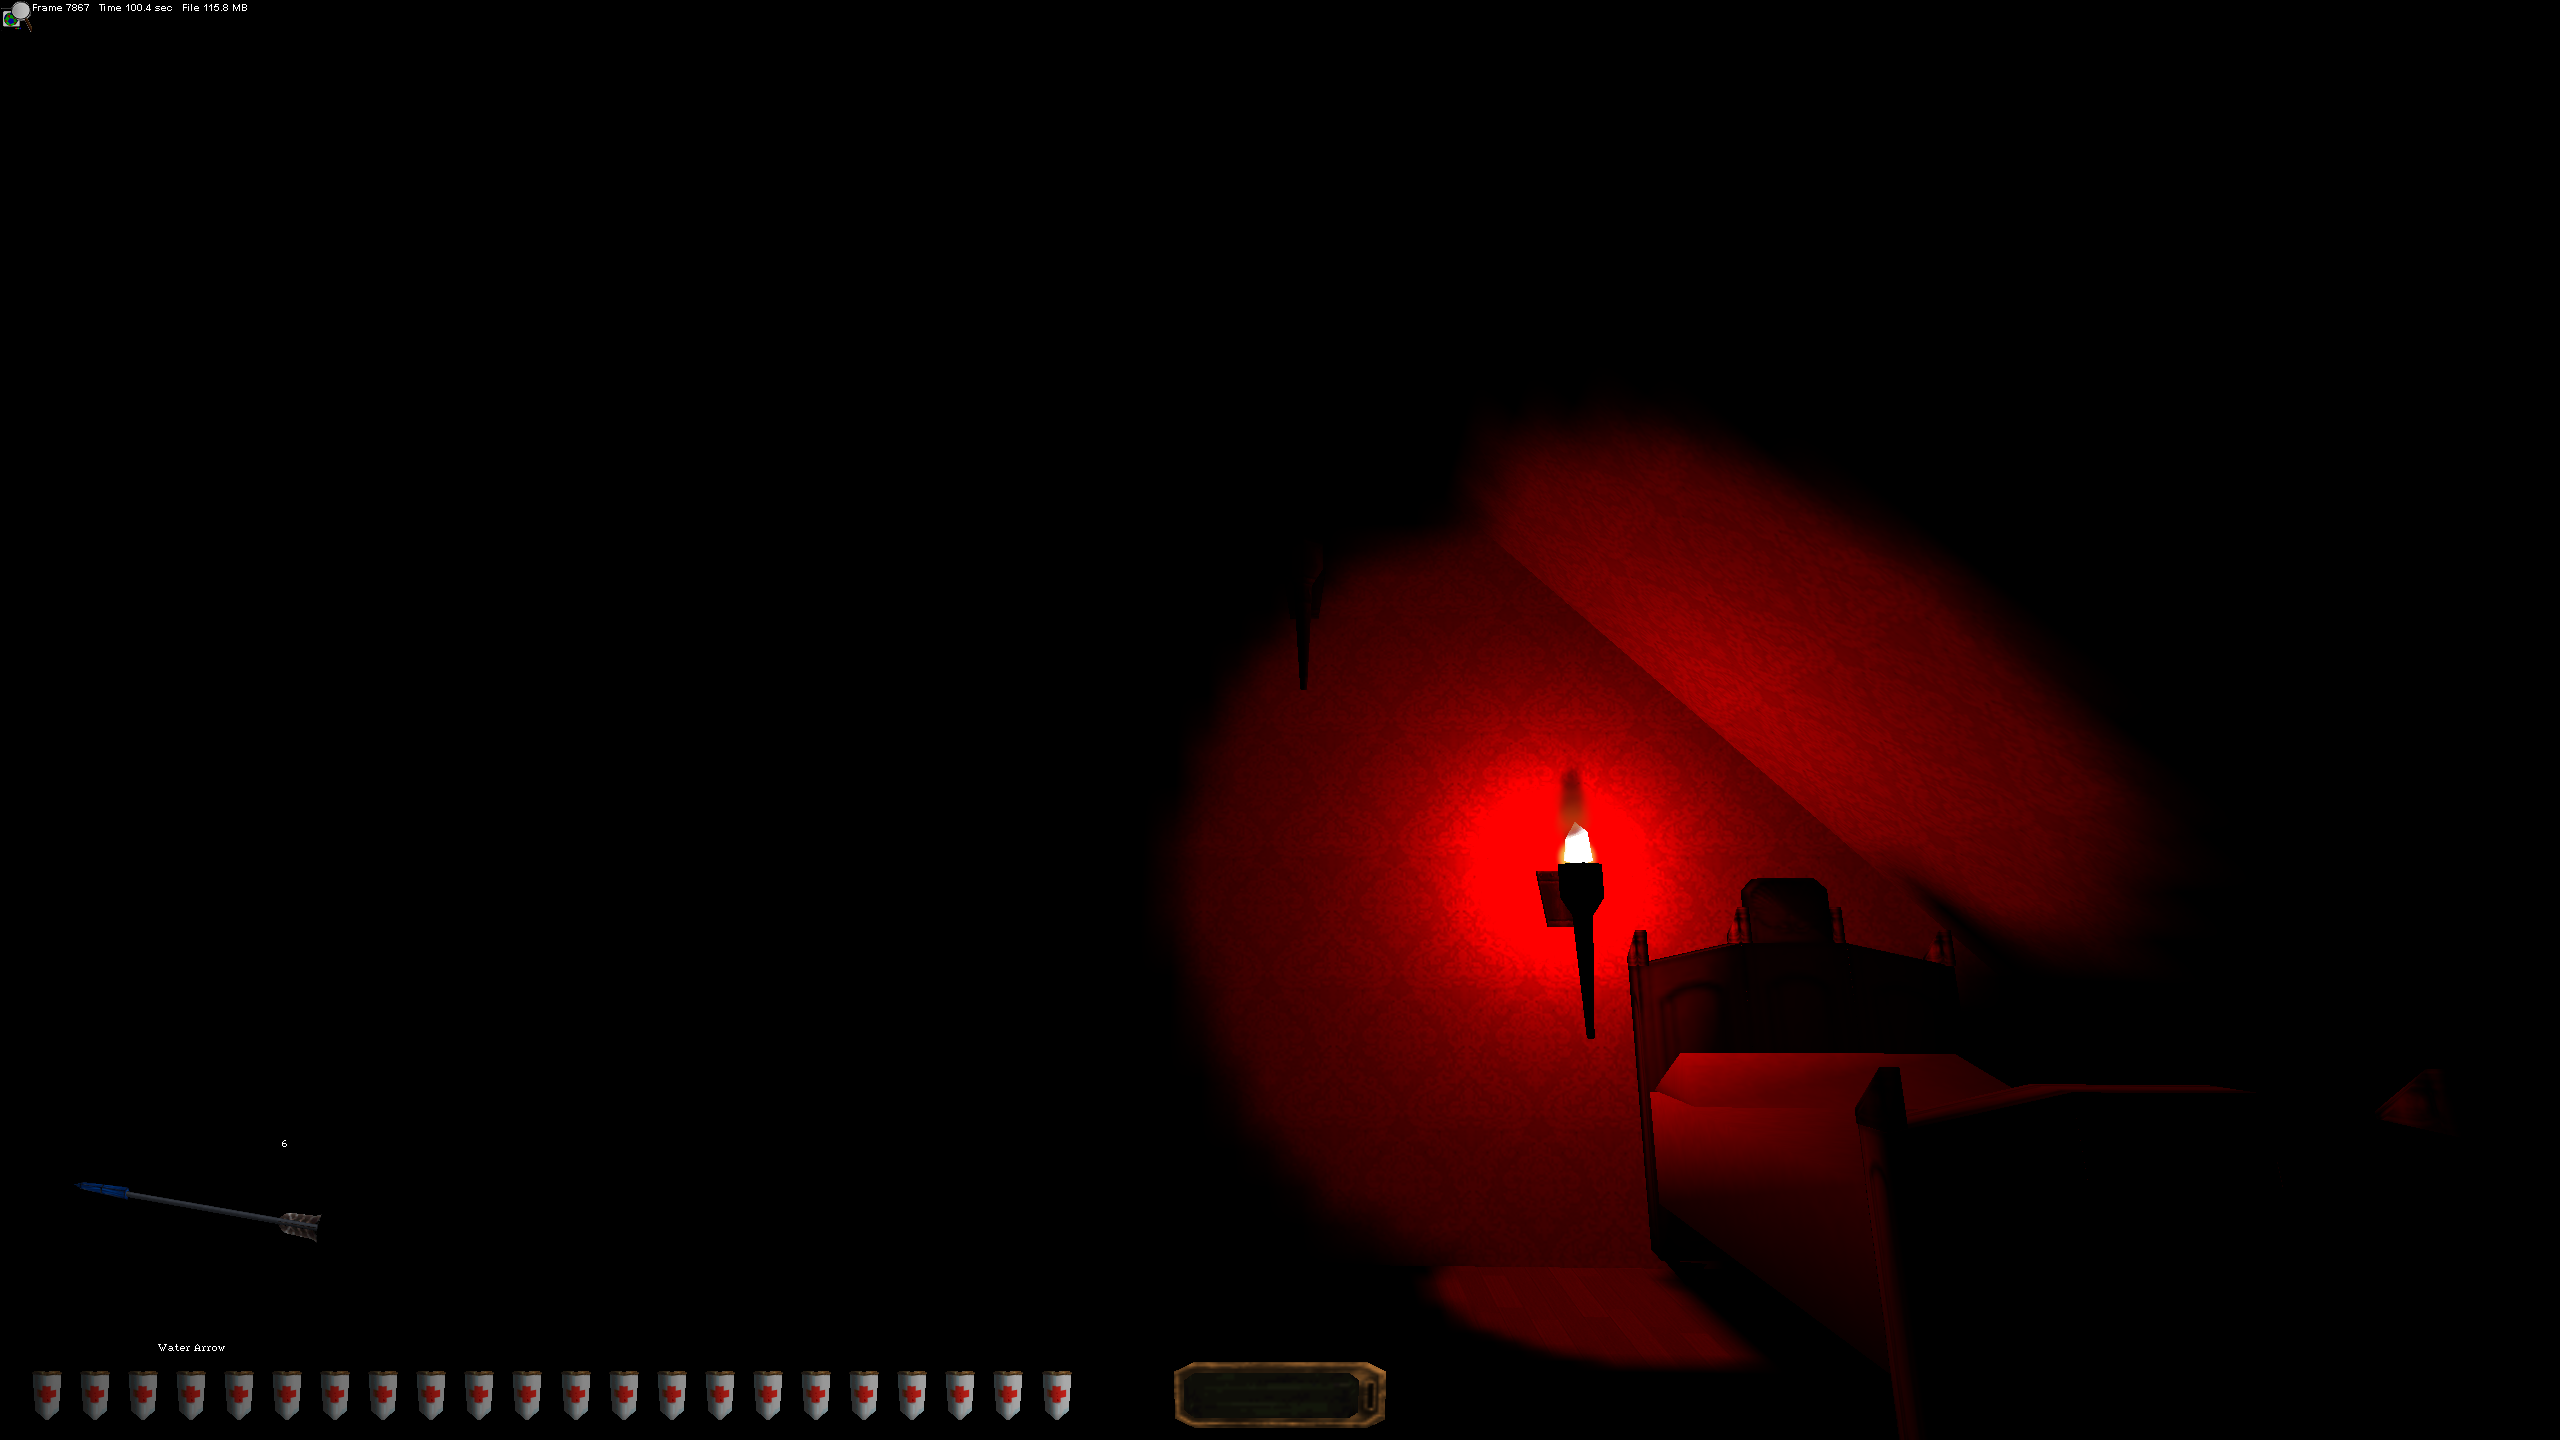
\includegraphics[width=1.00\textwidth]{img/PIX/render_r.png}
	\caption[Render of scene with the red torch lit]{Render of scene with the red torch lit}
	\label{fig:RenderR}
\end{figure}

%\setcounter{figure}{0}  
\clearpage
\counterwithin{figure}{section}
\counterwithin{listing}{section}
\section{Lightmap and render - green torch lit} 


\begin{figure}[htbp]
	\centering
		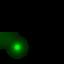
\includegraphics[width=0.40\textwidth]{img/PIX/g.png}
	\caption[Lightmap of scene with the green torch lit]{Lightmap of scene with the green torch lit}
	\label{fig:LightmapG}
\end{figure}
\begin{figure}[htbp]
	\centering
		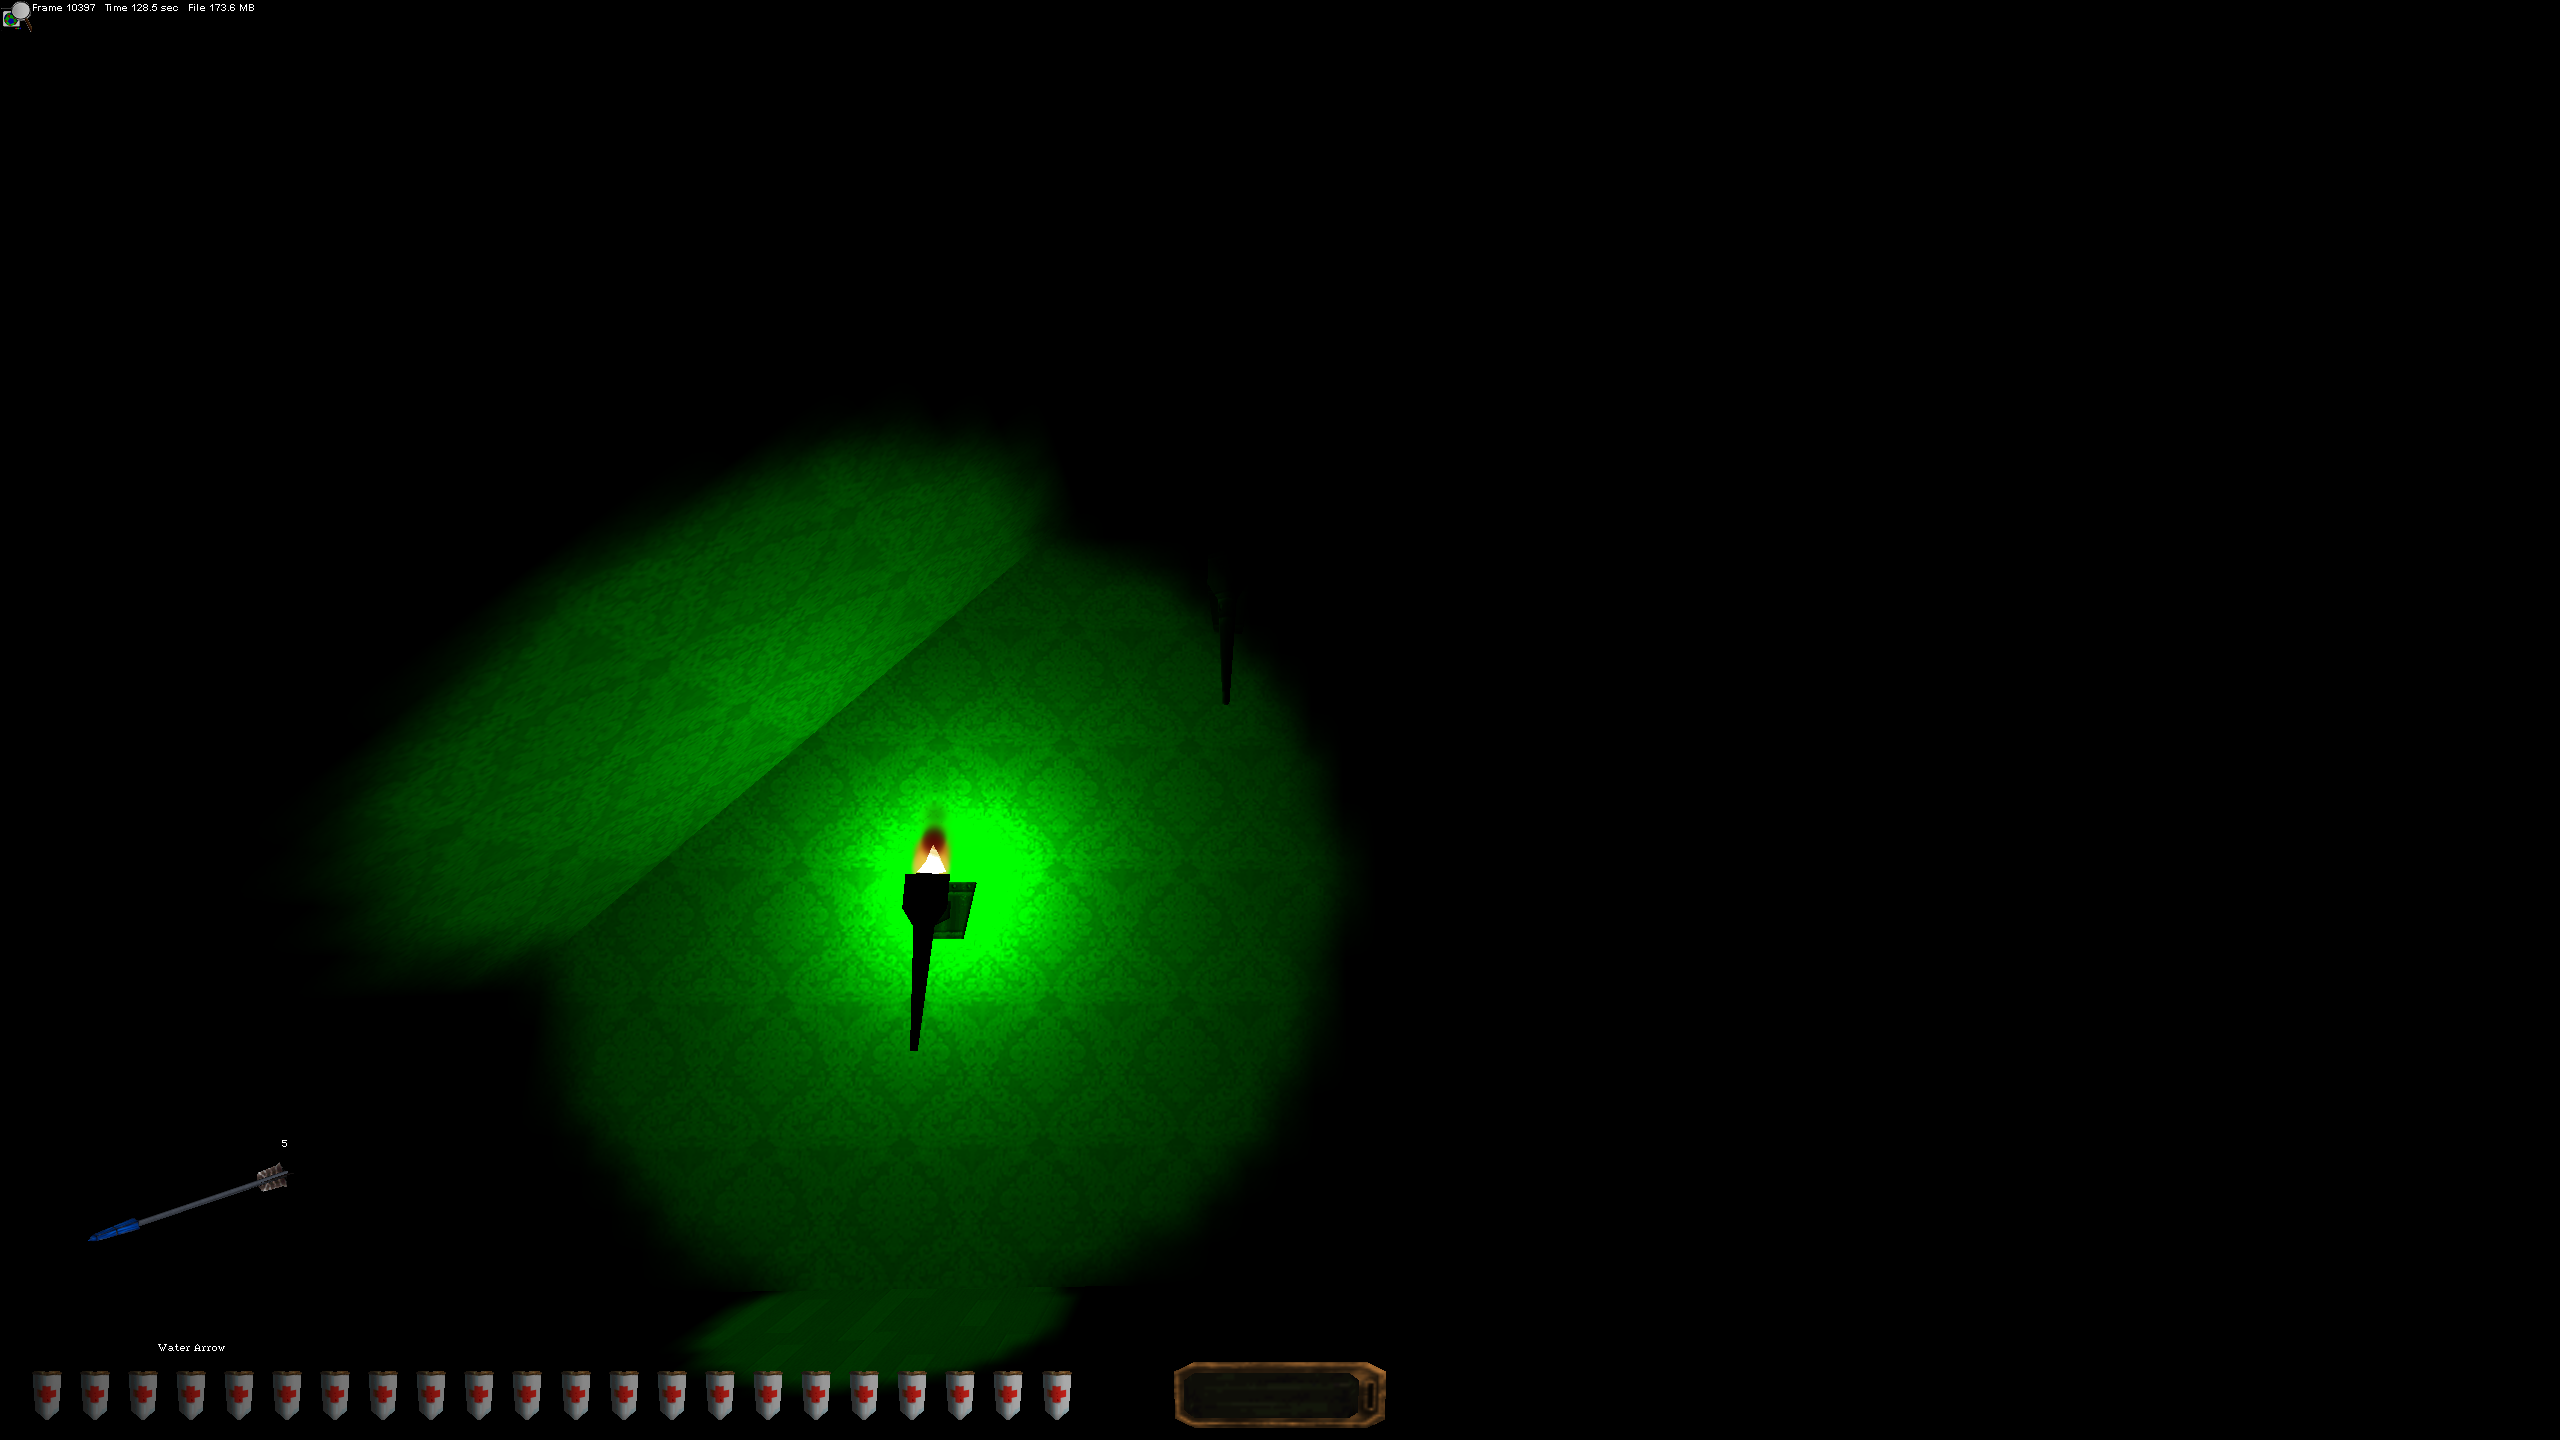
\includegraphics[width=1.00\textwidth]{img/PIX/render_g.png}
	\caption[Render of scene with the green torch lit]{Render of scene with the green torch lit}
	\label{fig:RenderG}
\end{figure}

%\setcounter{figure}{0}  
\clearpage
\counterwithin{figure}{section}
\counterwithin{listing}{section}
\section{Lightmap and render - blue torch lit} 

\begin{figure}[htbp]
	\centering
		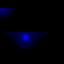
\includegraphics[width=0.40\textwidth]{img/PIX/b.png}
	\caption[Lightmap of scene with the blue torch lit]{Lightmap of scene with the blue torch lit}
	\label{fig:LightmapB}
\end{figure}
\begin{figure}[htbp]
	\centering
		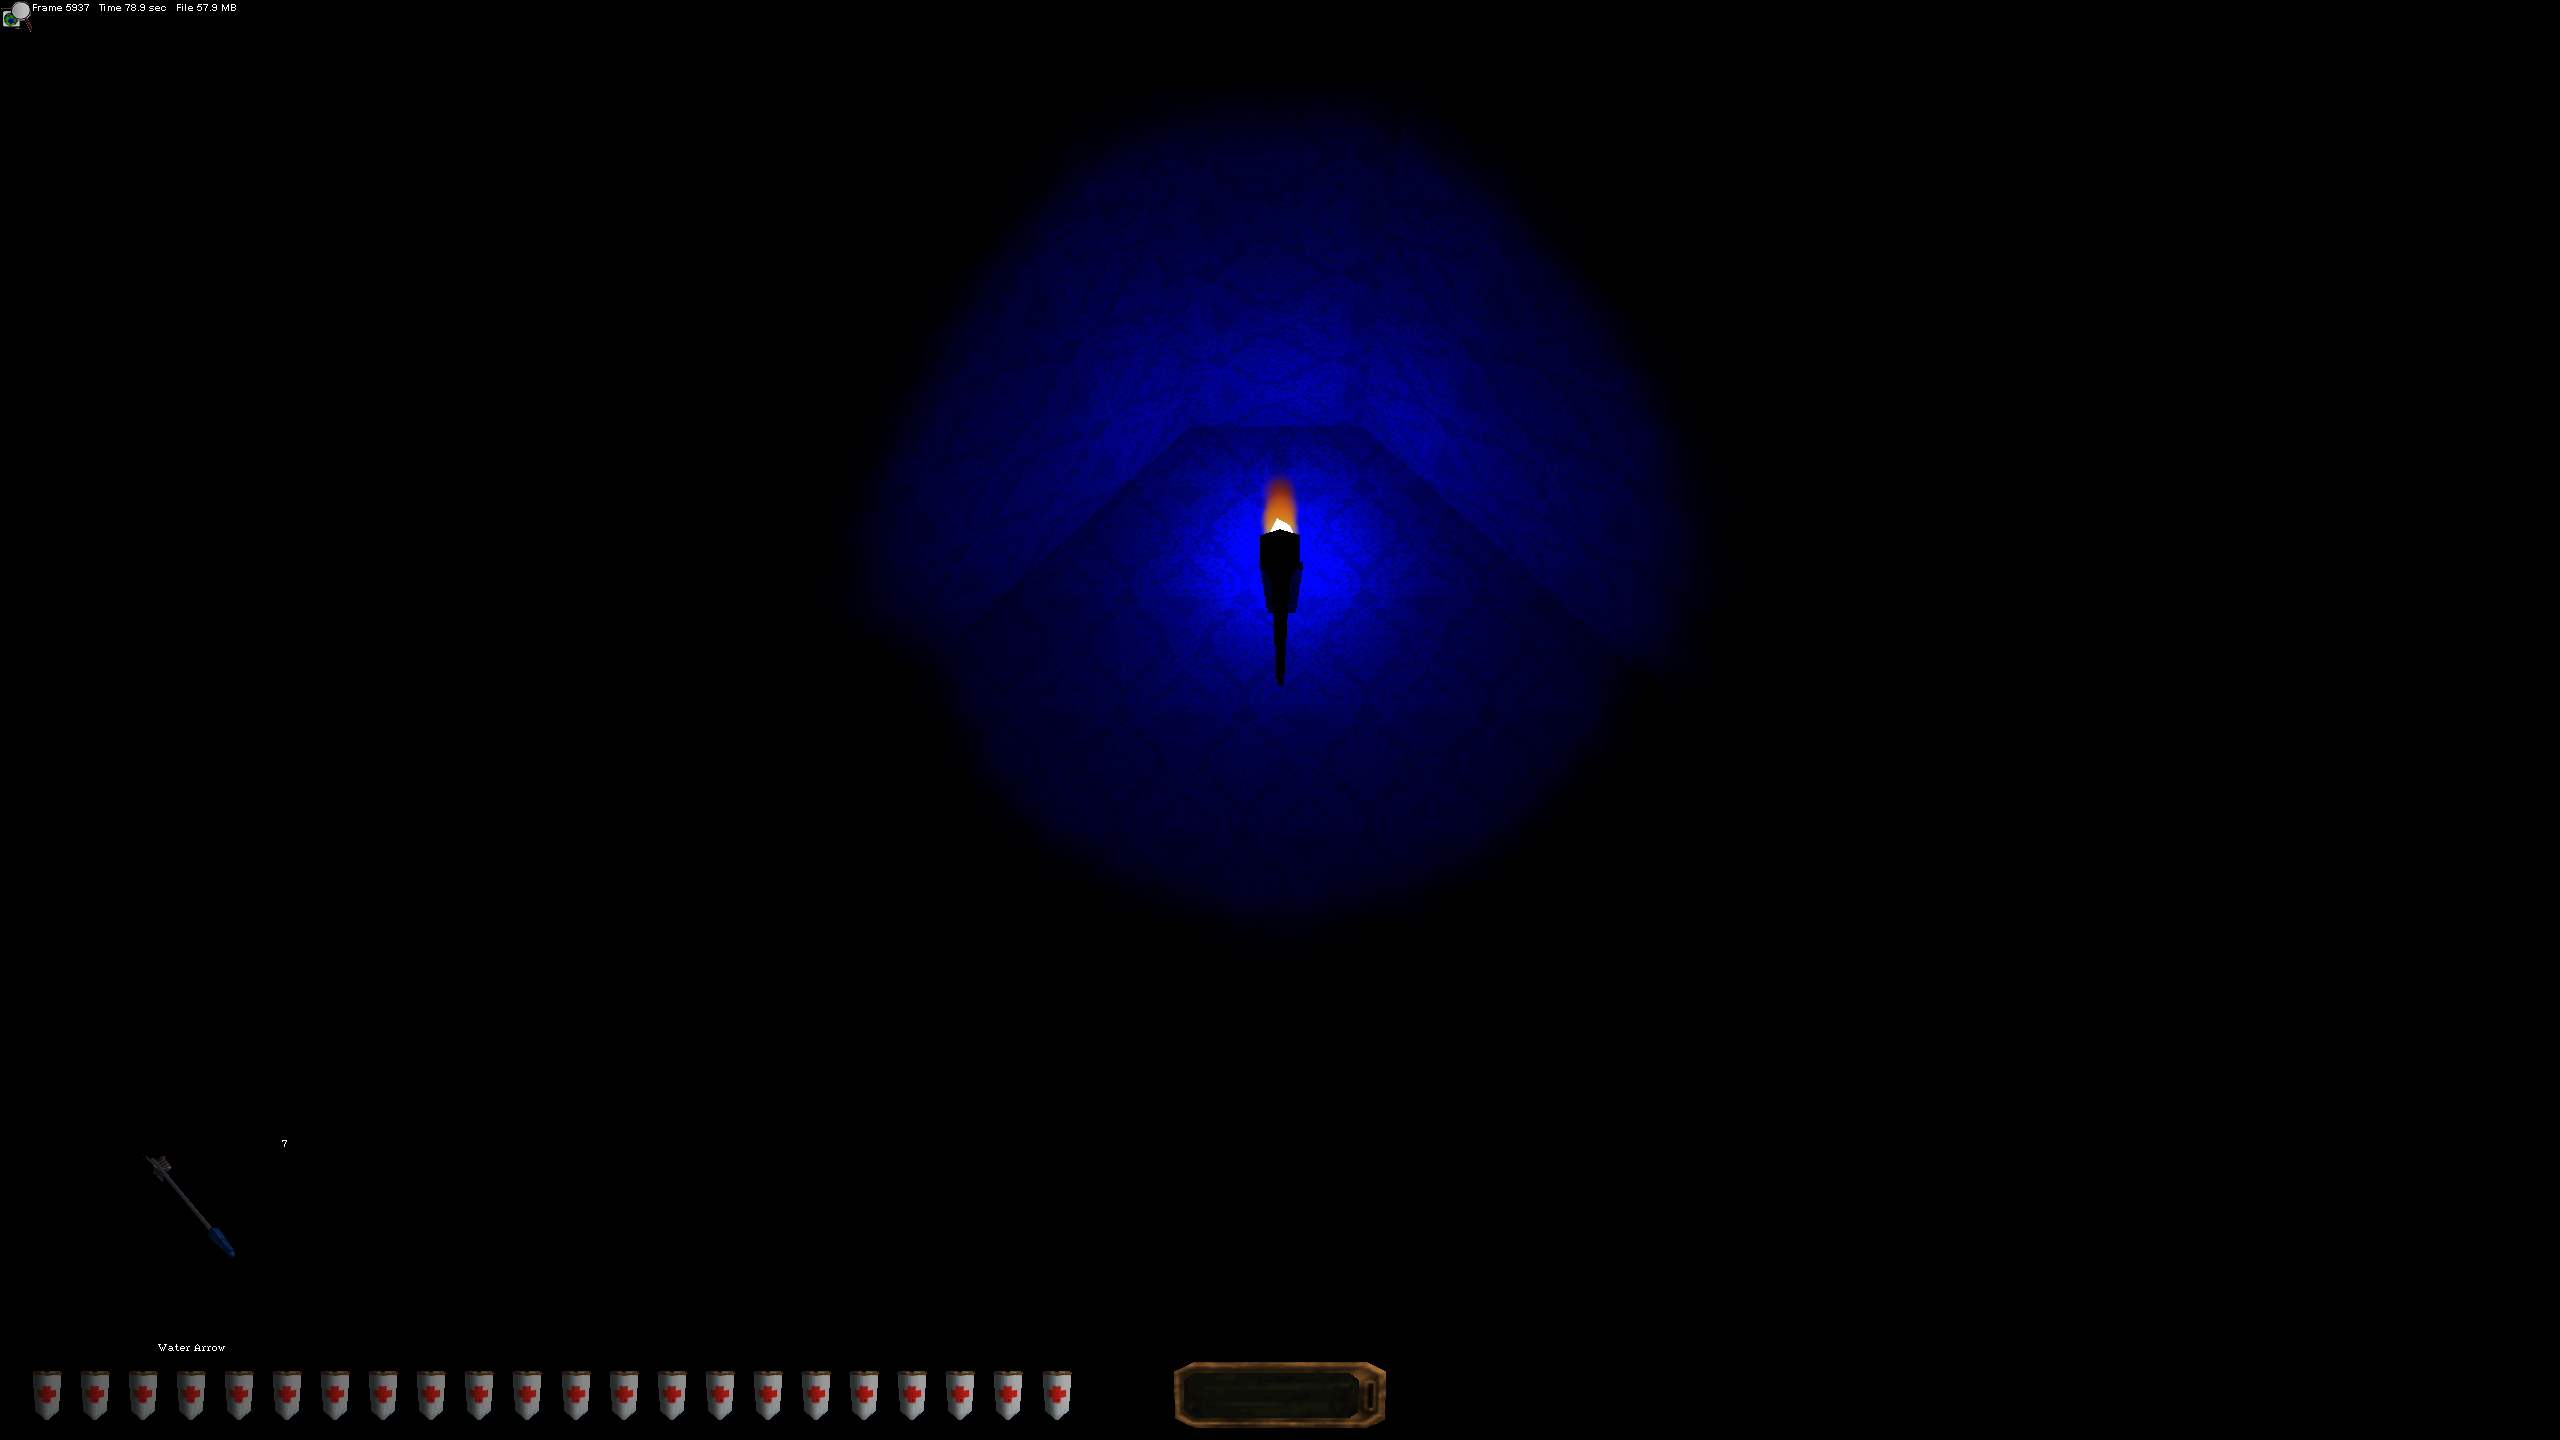
\includegraphics[width=1.00\textwidth]{img/PIX/render_b.png}
	\caption[Render of scene with the blue torch lit]{Render of scene with the blue torch lit}
	\label{fig:RenderB}
\end{figure}

%\setcounter{figure}{0}  
\clearpage
\counterwithin{figure}{section}
\counterwithin{listing}{section}
\section{Lightmap and render - no torch lit} 

\begin{figure}[htbp]
	\centering
		
\includegraphics[width=0.40\textwidth]{img/PIX/none.png}
	\caption[Lightmap of scene with no torch lit]{Lightmap of scene with no torch lit}
	\label{fig:LightmapNone}
\end{figure}
\begin{figure}[htbp]
	\centering
		
\includegraphics[width=1.00\textwidth]{img/PIX/render_none.png}
	\caption[Render of scene with no torch lit]{Render of scene with no torch lit}
	\label{fig:RenderNone}
\end{figure}


\end{appendix} 


\mbox{}
\newpage




%\setcounter{secnumdepth}{0} % Hide Section number in toc (If not: A Eidesstattliche Erklärung)

%\includepdf[pages={1},addtotoc={
%     1,section,1,Eidesstattliche Erkl\"arung,p1}]{EidesstattlicheErklaerung.pdf}

% Eidesstattliche Erklärung ununterschrieben
%\clearpage
%\section*{Eidesstattliche Erklärung}
%\addcontentsline{toc}{section}{Eidesstattliche Erklärung}%\addtocontents{toc}{\vfill}
%Ich versichere, dass ich die vorstehende Arbeit selbständig angefertigt und mich fremder Hilfe nicht bedient habe. Alle Stellen, die wörtlich oder sinngemäß veröffentlichtem oder nicht veröffentlichtem Schrifttum entnommen sind, habe ich als solche kenntlich gemacht.\\\\

%\noindent Wernigerode, den 01.02.2019
%\begin{flushright}
%$\overline{~~~~~~~~~\mbox{Alexander Johr}~~~~~~~~~}$
%\end{flushright}
%\mbox{}


\end{document}
 